\section{مسارات الموافقة}
\label{sec:settings-feature-approval-routes}

المسار وصف محفوظ لمن يجب أن يوافق، وبأي ترتيب، وماذا يحدث عند التأخر. تبنيه مرة واحدة في هذه الصفحة، ثم تستخدمه الانتقالات والنماذج وطلبات الموافقة وقواعد المناقلة، فلا تعيد بناء الموافقات نفسها في كل مكان. يطّلع على المسارات من يملك صلاحية ذلك، أما تغييرها فيحتاج إلى صلاحية إدارة مسارات الموافقة.

\begin{rcnote}[مثال: شركة الأفق]
يضغط مسؤول النظام «مسار جديد» عند ① لبناء مسار «موافقة المشتريات»: يوافق عمر حداد أولاً، ثم المدير العام. وبعد النشر يتابع الطلبات الجارية من ⑤ قبل أي تعديل لاحق.
\end{rcnote}

\begin{figure}[H]
\centering
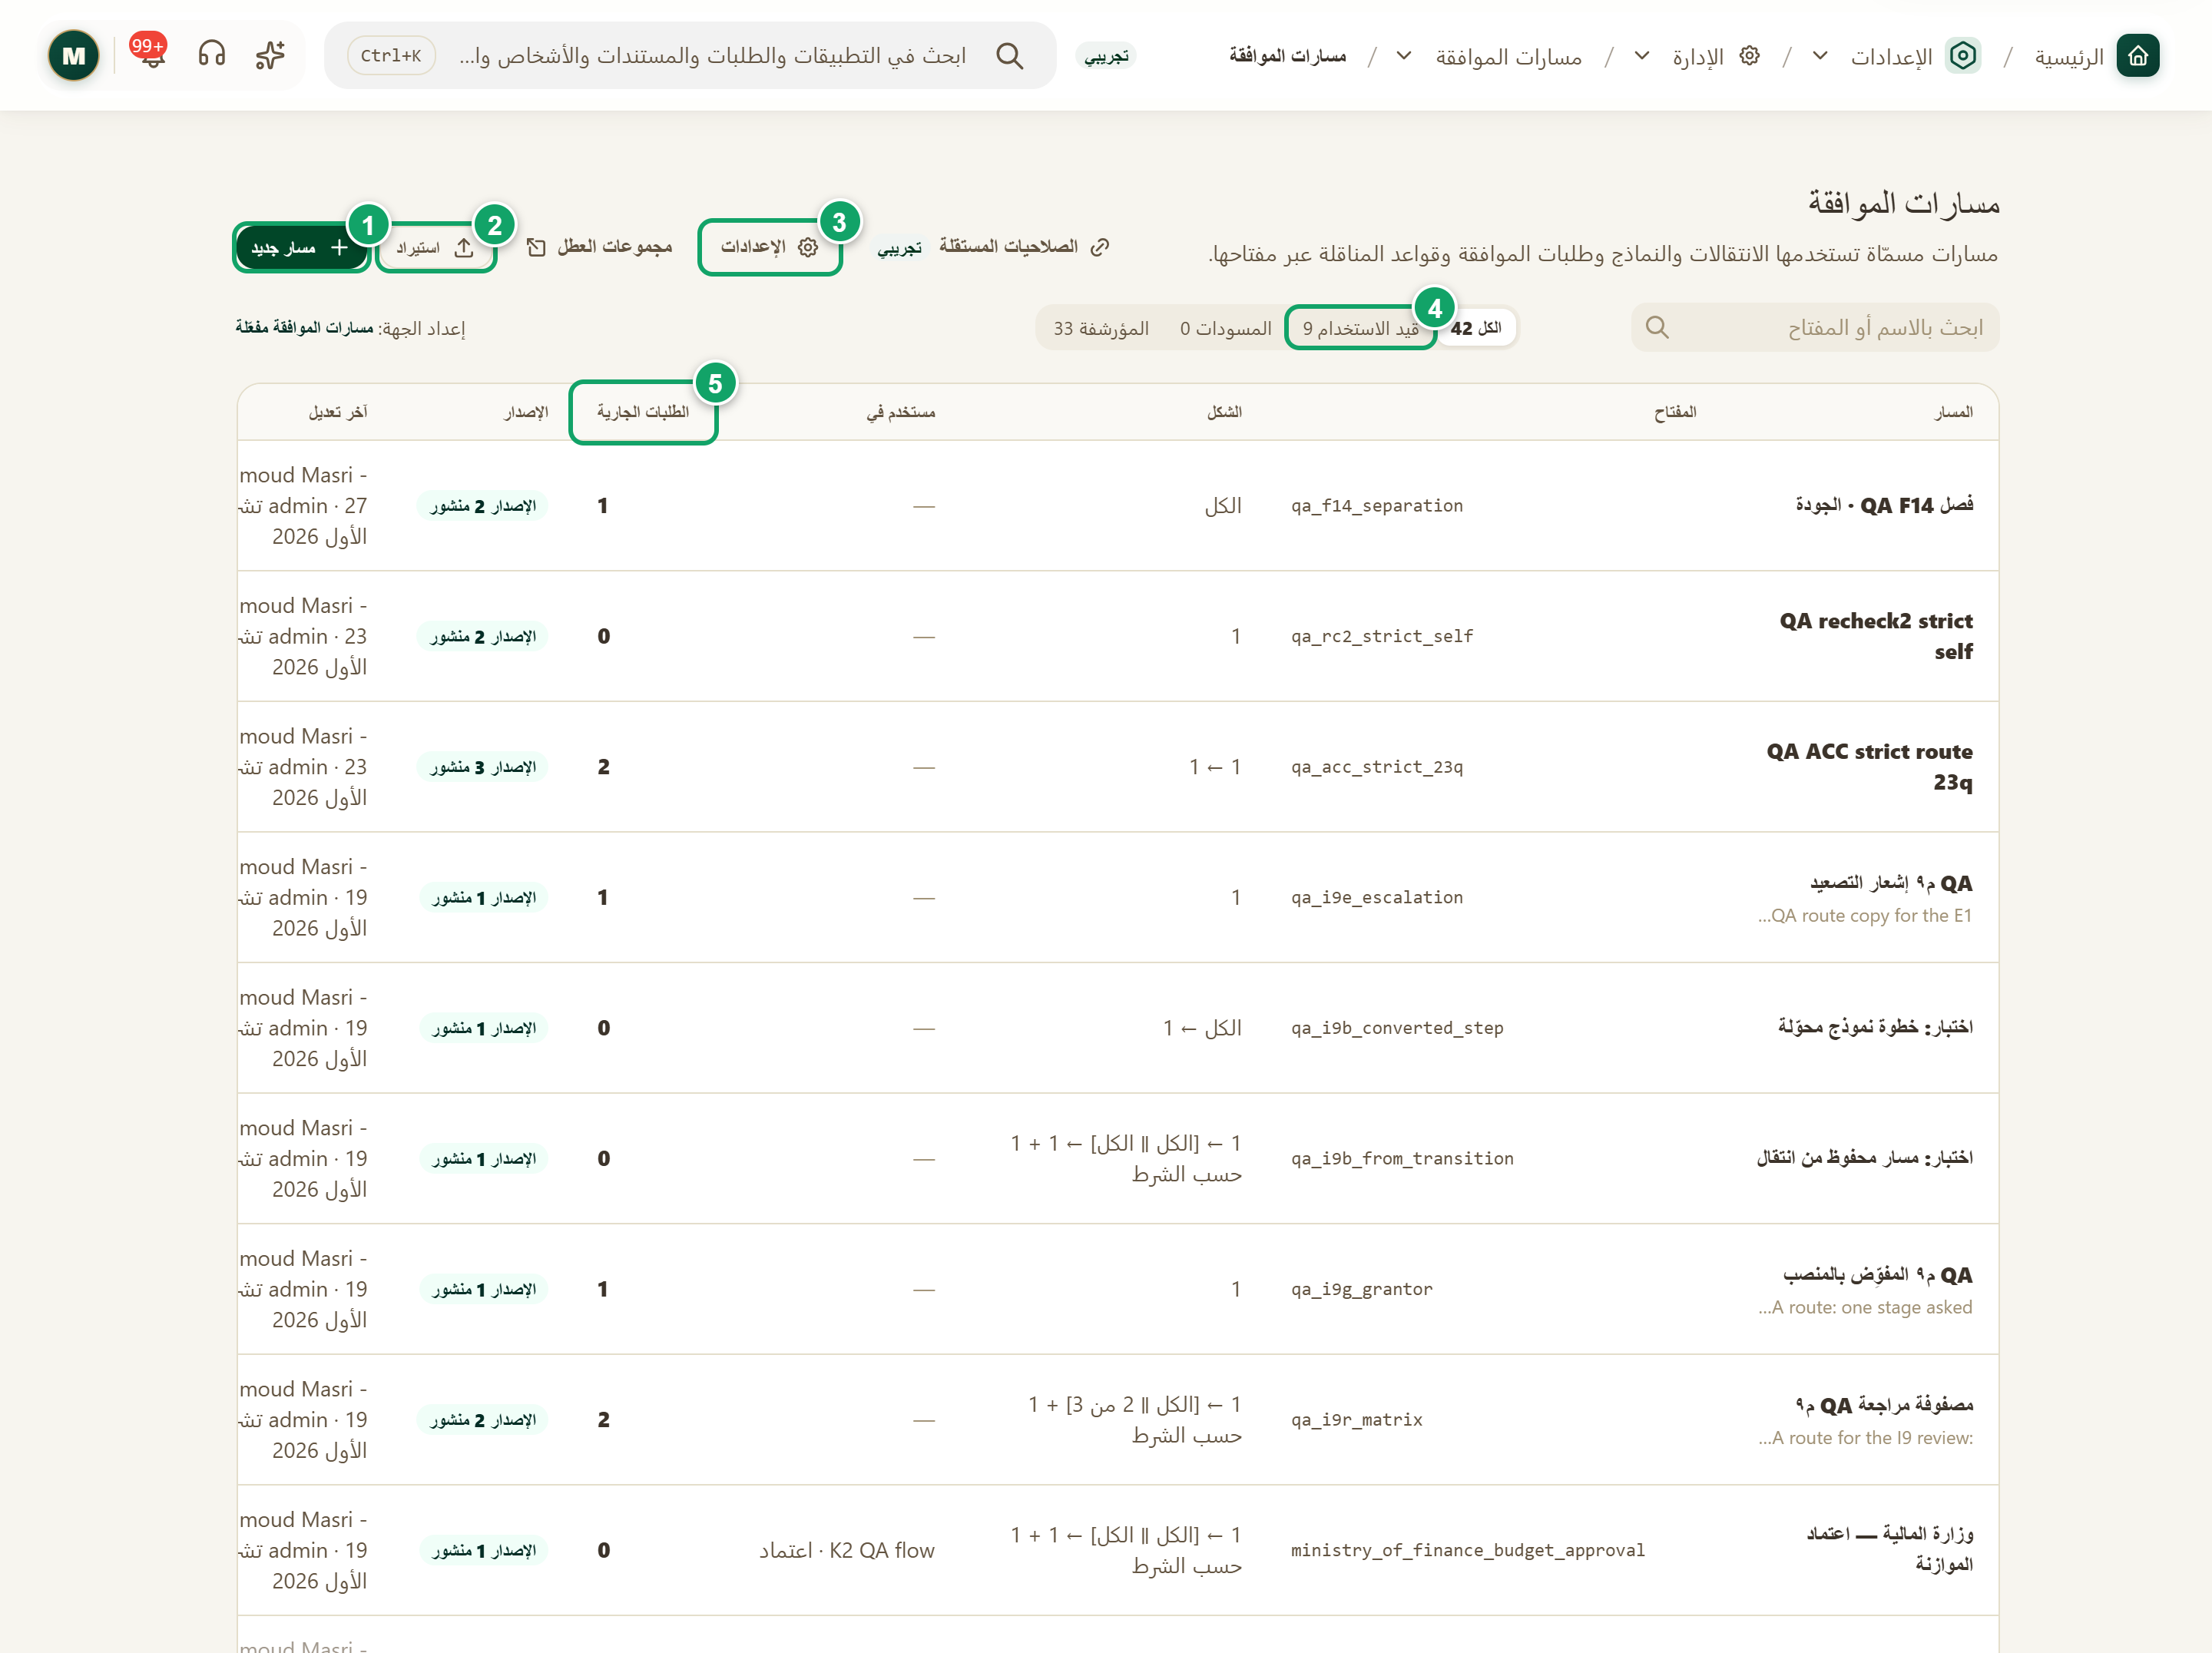
\includegraphics[width=0.95\linewidth,height=0.72\textheight,keepaspectratio]{figures/screens/ch08-approval-routes-ar.png}
\caption{مكتبة مسارات الموافقة}
\label{fig:settings-approval-routes-screen}
\shotnote{تجمع المكتبة مسارات المؤسسة، ويختصر عمود «الشكل» ترتيب موافقات كل مسار، ويبين عمود «مستخدم في» المكان الذي يعتمد عليه. والمسارات الظاهرة مسارات اختبار. ① «مسار جديد». ② «استيراد»: يضيف ملف مسار مصدَّراً كمسودة. ③ «الإعدادات»: مفتاح التفعيل وتقويم العمل. ④ «قيد الاستخدام»: لتصفية المسارات المستخدمة. ⑤ «الطلبات الجارية»: عدد الطلبات التي تسير الآن على المسار.}
\end{figure}

\begin{figure}[H]
\centering
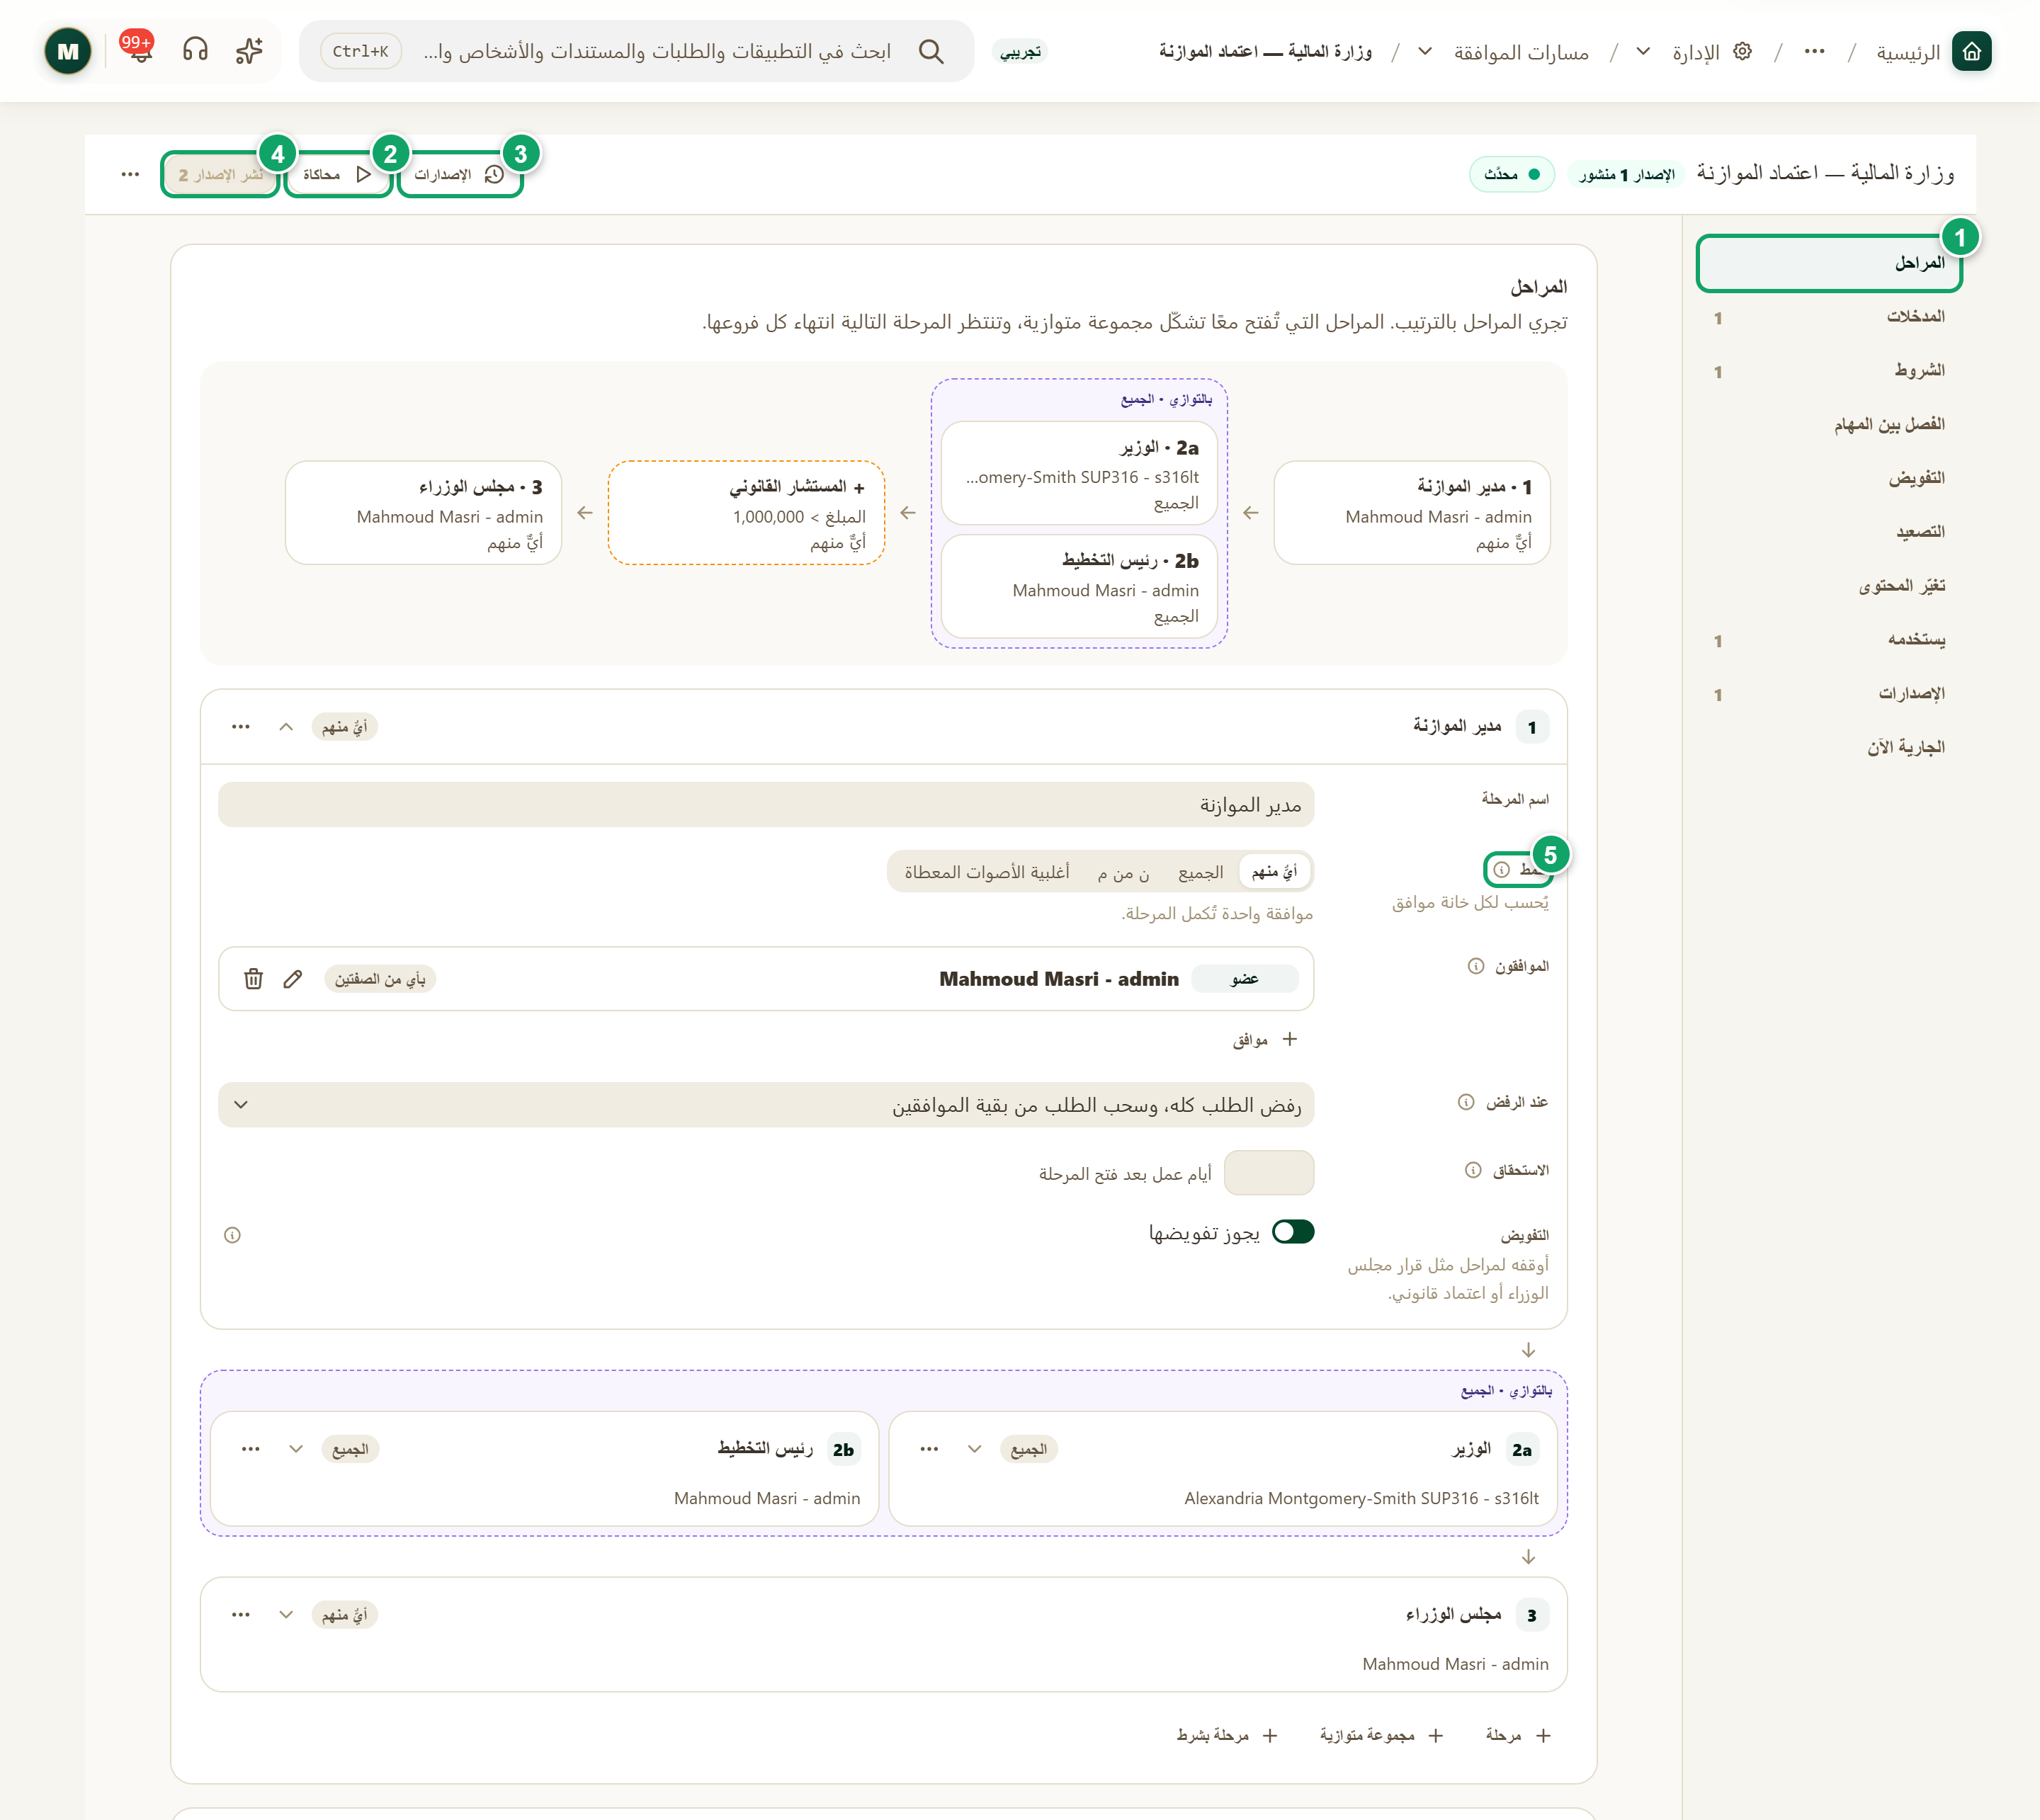
\includegraphics[width=0.95\linewidth,height=0.72\textheight,keepaspectratio]{figures/screens/ch08-approval-routes-editor-ar.png}
\caption{محرر المسار: المراحل}
\label{fig:settings-approval-routes-editor-screen}
\shotnote{يعرض المحرر شكل المسار كاملاً، ثم تفاصيل كل مرحلة. أما بقية أقسام المسار فيشرحها الجدول التالي. ① «المراحل»: قائمة الأقسام. ② «محاكاة»: تجرب المسار بقيم تجريبية، ولا تحفظ شيئاً ولا ترسل إشعاراً. ③ «الإصدارات». ④ «نشر الإصدار»: يعمل عند وجود تغييرات في المسودة دون أخطاء. ⑤ «النمط»: عدد الموافقات التي تُكمل المرحلة.}
\end{figure}

\begin{table}[H]
\centering
\caption{ماذا تسجل في المسار؟}
\label{tab:settings-approval-routes-fields}
\begin{tabularx}{\linewidth}{R{4.2cm} Y}
\rcHeaderRow
\thh{القسم} & \thh{ماذا تحدد فيه؟}\\
«المراحل» & اسم كل مرحلة و«النمط»: «أيٌّ منهم» أو «الجميع» أو «ن من م» أو «أغلبية الأصوات المعطاة». ثم «الموافقون» (عضو أو منصب أو دور أو تعبير أو مصفوفة الصلاحيات)، و«عند الرفض»، و«الاستحقاق». ويمكن تشغيل مراحل بالتوازي.\\
«المدخلات» & قيم يربطها كل مكان استخدام بحقوله، مثل المبلغ، ليصلح المسار لأنواع سجلات مختلفة.\\
«الشروط» & قواعد تضيف مراحل عند تحققها، مثل مستشار قانوني إذا تجاوز المبلغ حداً معيناً.\\
«الفصل بين المهام» & من يحق له القرار: منع صاحب الطلب من الموافقة، وعدم تكرار قرار الشخص نفسه، واشتراط التوقيع، والسماح بإعادة الطلب للتعديل.\\
«التفويض» & هل يجوز تسليم الدور لشخص آخر لمدة محددة، ولمن، وهل يوقّع المفوَّض إليه.\\
«التصعيد» & تقويم الأيام، والمهلة الافتراضية، وخطوات تنبيه المتأخرين. ولا يوافق النظام أو يرفض من تلقاء نفسه.\\
«تغيّر المحتوى» & مصير الموافقات إذا تغيّر السجل أثناء سير المسار: تبقى، أو يعاد المسار كله، أو يعاد من المرحلة المتأثرة.\\
«يستخدمه» و«الإصدارات» و«الجارية الآن» & أماكن الاستخدام، والإصدارات المنشورة، والطلبات التي تسير الآن.\\
\end{tabularx}
\end{table}

الإصدار نسخة منشورة لا تتغير. تُحفظ تعديلاتك تلقائياً في مسودة لا تؤثر في أي طلب حتى تنشرها، ويسجل كل طلب الإصدار الذي بدأ عليه.

\begin{figure}[H]
\centering
\begin{tikzpicture}[node distance=0.5cm]
\node[stepBox] (a) {\RL{تُحفظ التعديلات في مسودة}};
\node[stepBox,below=of a] (b) {\RL{يضغط المسؤول «نشر الإصدار»}};
\node[stepBox,below=of b] (c) {\RL{تبدأ الطلبات الجديدة على الإصدار الجديد}};
\node[stepBox,below=of c] (d) {\RL{تبدأ أي تعديلات لاحقة مسودة جديدة}};
\draw[flowsTo] (a) -- (b);
\draw[flowsTo] (b) -- (c);
\draw[flowsTo] (c) -- (d);
\end{tikzpicture}
\rclegend
\caption{من المسودة إلى إصدار منشور}
\label{fig:settings-approval-routes-versions}
\shotnote{يبين المخطط لماذا يكون تعديل المسار آمناً: فالنشر هو الخطوة التي تجعل التعديل فعّالاً. أما الطلبات التي بدأت قبل النشر فتكمل على إصدارها القديم، لذلك لا تتوقع أن يصلها التغيير.}
\end{figure}

\begin{figure}[H]
\centering
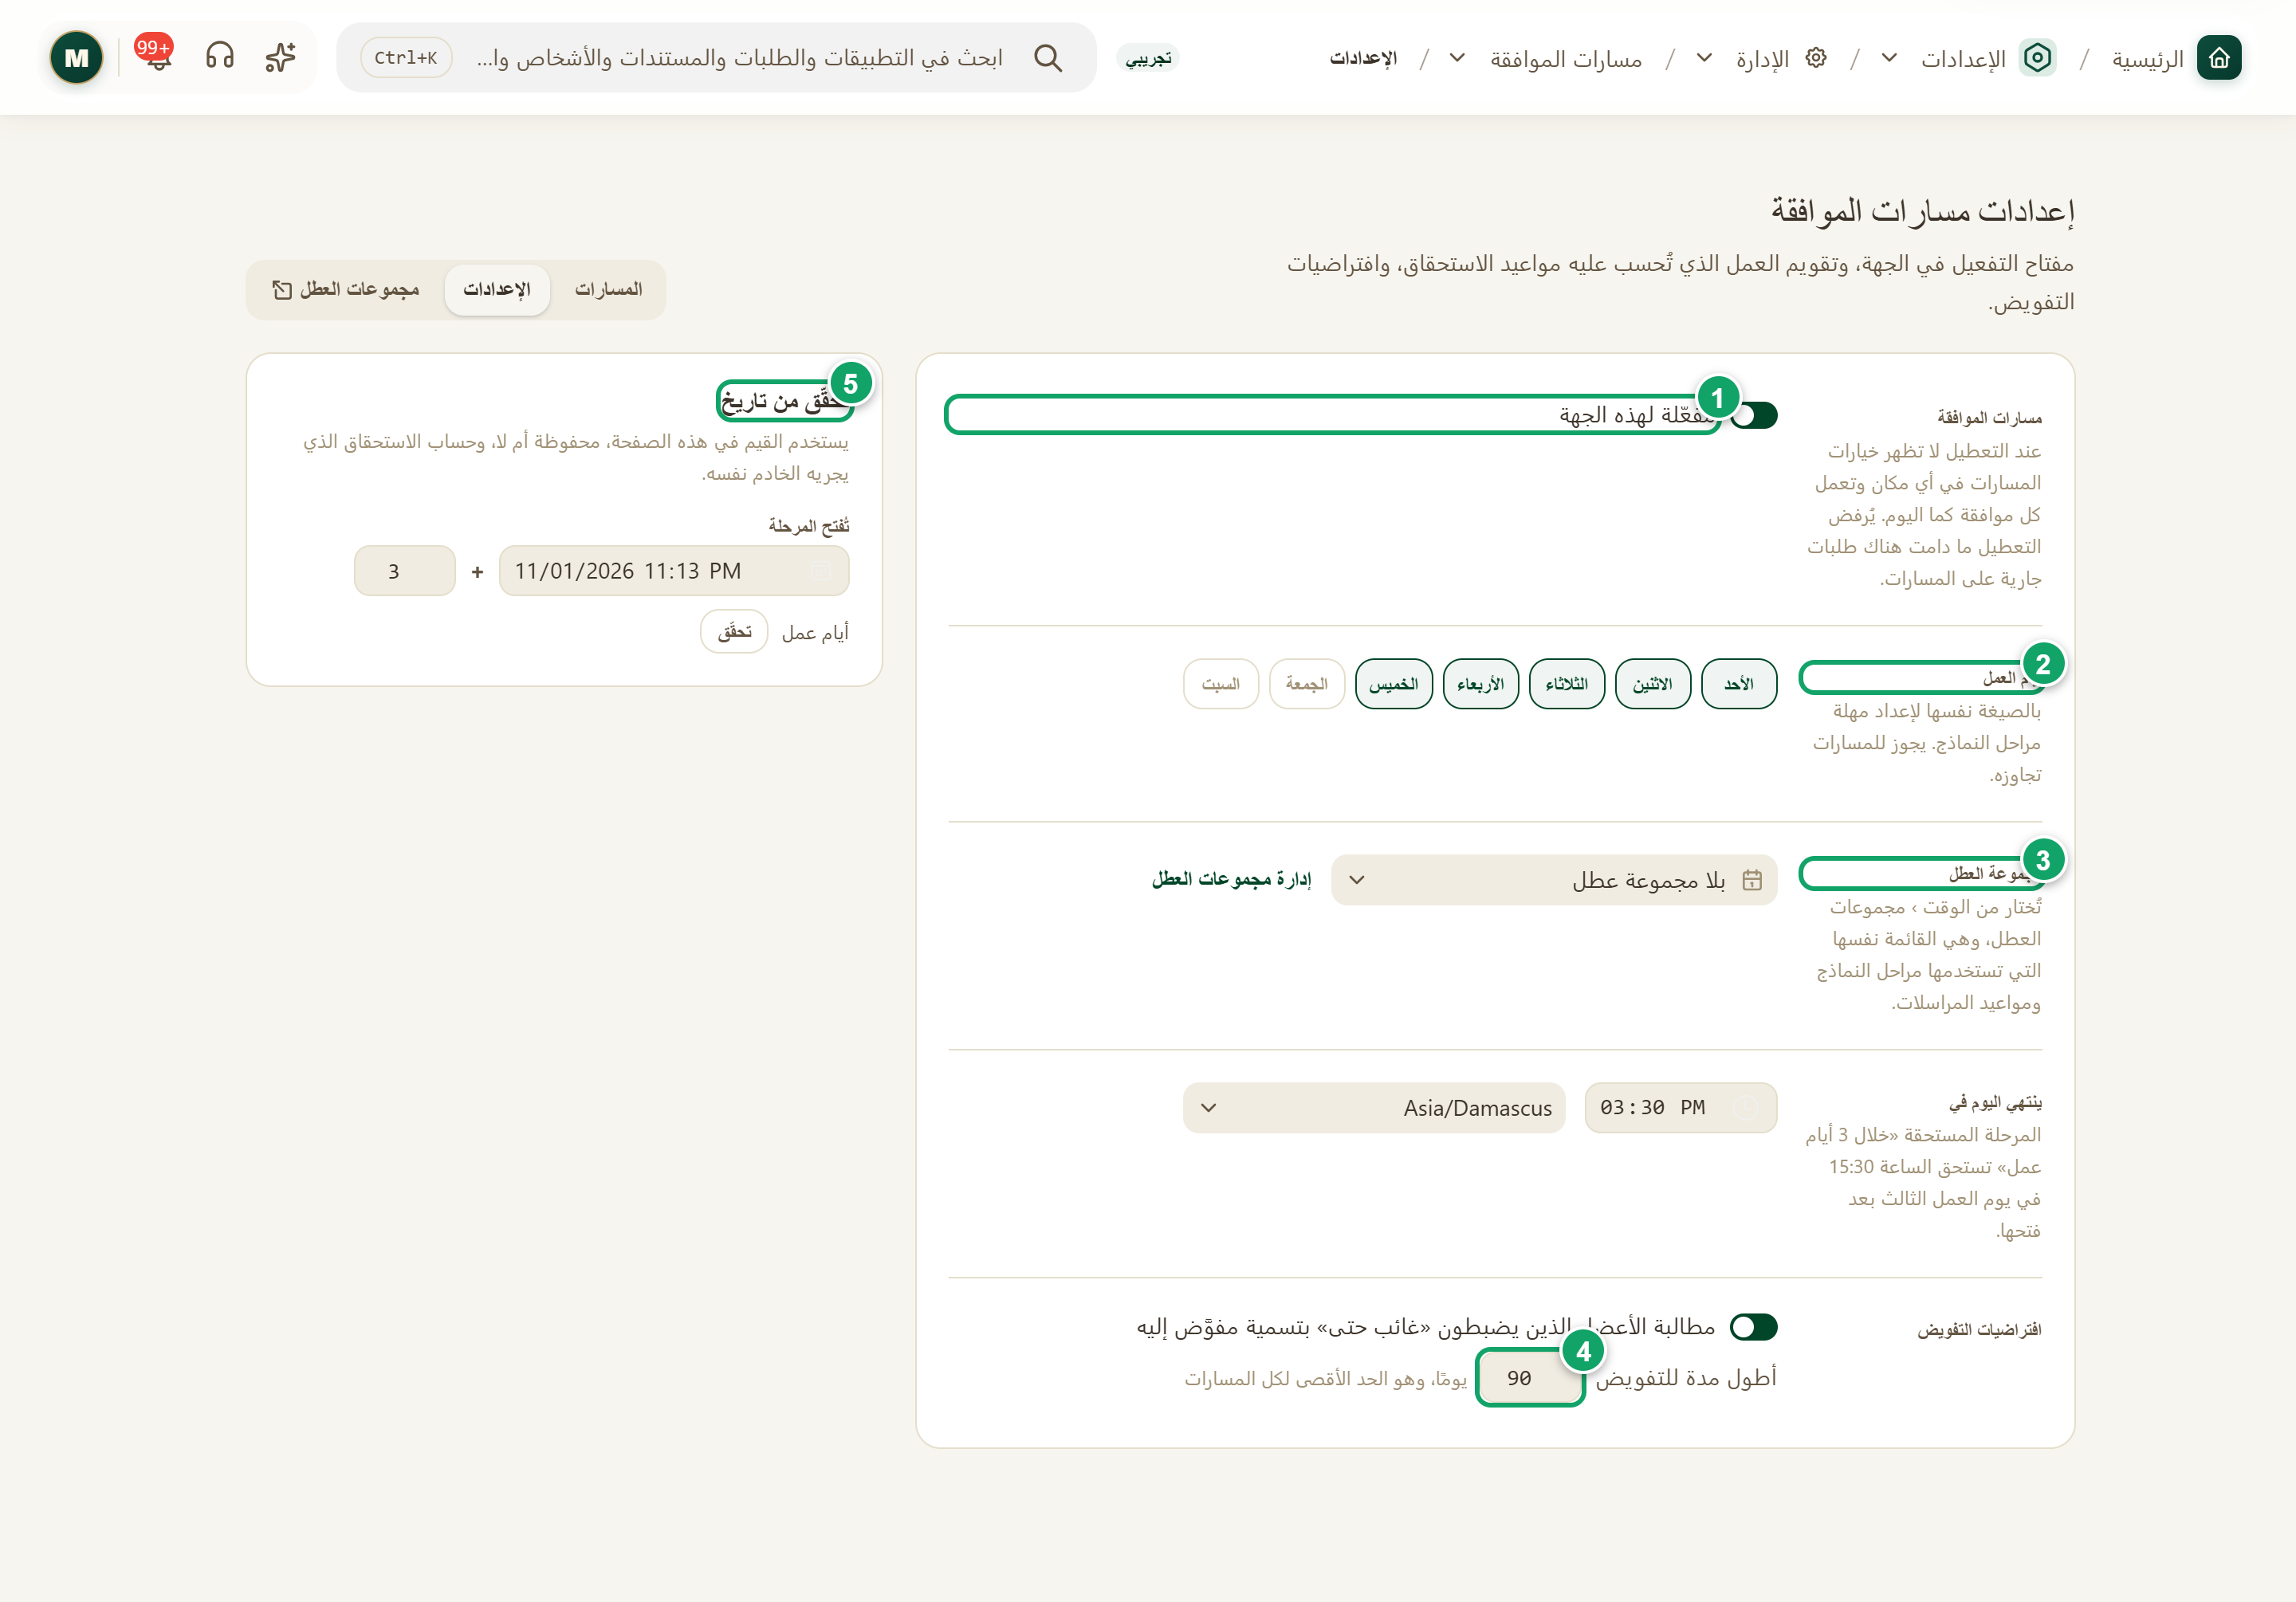
\includegraphics[width=0.95\linewidth,height=0.72\textheight,keepaspectratio]{figures/screens/ch08-approval-routes-settings-ar.png}
\caption{إعدادات مسارات الموافقة}
\label{fig:settings-approval-routes-settings-screen}
\shotnote{تجمع الصفحة قرارات تسري على كل المسارات، وأهمها تقويم العمل الذي تُحسب عليه مواعيد الاستحقاق. ويمكنك تجربة التقويم قبل حفظه. ① «مفعّلة لهذه الجهة»: عند التعطيل تختفي خيارات المسارات، ويُرفض التعطيل ما دامت هناك طلبات جارية. ② «أيام العمل». ③ «مجموعة العطل». ④ «أطول مدة للتفويض». ⑤ «تحقّق من تاريخ»: يحسب موعد الاستحقاق من تاريخ فتح المرحلة.}
\end{figure}

\begin{enumerate}
\item افتح «الإعدادات» ثم «مسارات الموافقة»، وتأكد من ظهور «مسارات الموافقة مفعّلة».
\item اضغط «مسار جديد»، واكتب العنوان والمفتاح، ثم اضغط «إنشاء المسار». لا يتغير المفتاح بعد ذلك.
\item أضف المراحل، ثم حدد لكل مرحلة «النمط» و«الموافقون»، وراجع بقية الأقسام.
\item اضغط «محاكاة» لتجربة المسار، ثم صحّح المشكلات؛ فالأخطاء تمنع النشر والتحذيرات لا تمنعه.
\item اضغط «نشر الإصدار» وأكد، ثم اختر المسار من الانتقال أو النموذج أو الطلب الذي يحتاج إليه.
\end{enumerate}

\textbf{تحقق:} يظهر المسار بشارة الإصدار المنشور، ويظهر مكان استخدامه تحت «يستخدمه». لا يمكن حذف مسار مستخدم أو منشور؛ فإذا انتهت الحاجة إليه، انقل مستخدميه إلى مسار آخر ثم اضغط «أرشفة». ويقتصر «حذف المسودة» على مسار لم يُنشر.

\section{قوالب التقييم}
\label{sec:settings-feature-evaluation-templates}

قالب التقييم بطاقة تستخدمها أكثر من مرة: معايير، ونموذج درجات، وفئات اختيارية تحوّل المجموع إلى نتيجة موصى بها. تختار أنواع السجلات قالباً لكل نوع من التقييم، مثل تقييم المورد أو المقابلة، فيقيّم الجميع بالمعايير نفسها. ويستطيع القراءة من يملك صلاحية تعديل الكيانات أو صلاحية إدارة القوالب، أما التعديل والنشر فلكل منهما صلاحية مستقلة.

\begin{rcnote}[مثال: شركة الأفق]
يضغط مسؤول النظام «قالب جديد» عند ① لإنشاء قالب «تقييم مورد الضيافة» من قالب في «حزمة المشتريات» عند ②. ثم يضيف شرطاً إلزامياً لوجود سجل تجاري، وينشر الإصدار ليستخدمه عمر حداد عند تقييم الموردين.
\end{rcnote}

\begin{figure}[H]
\centering
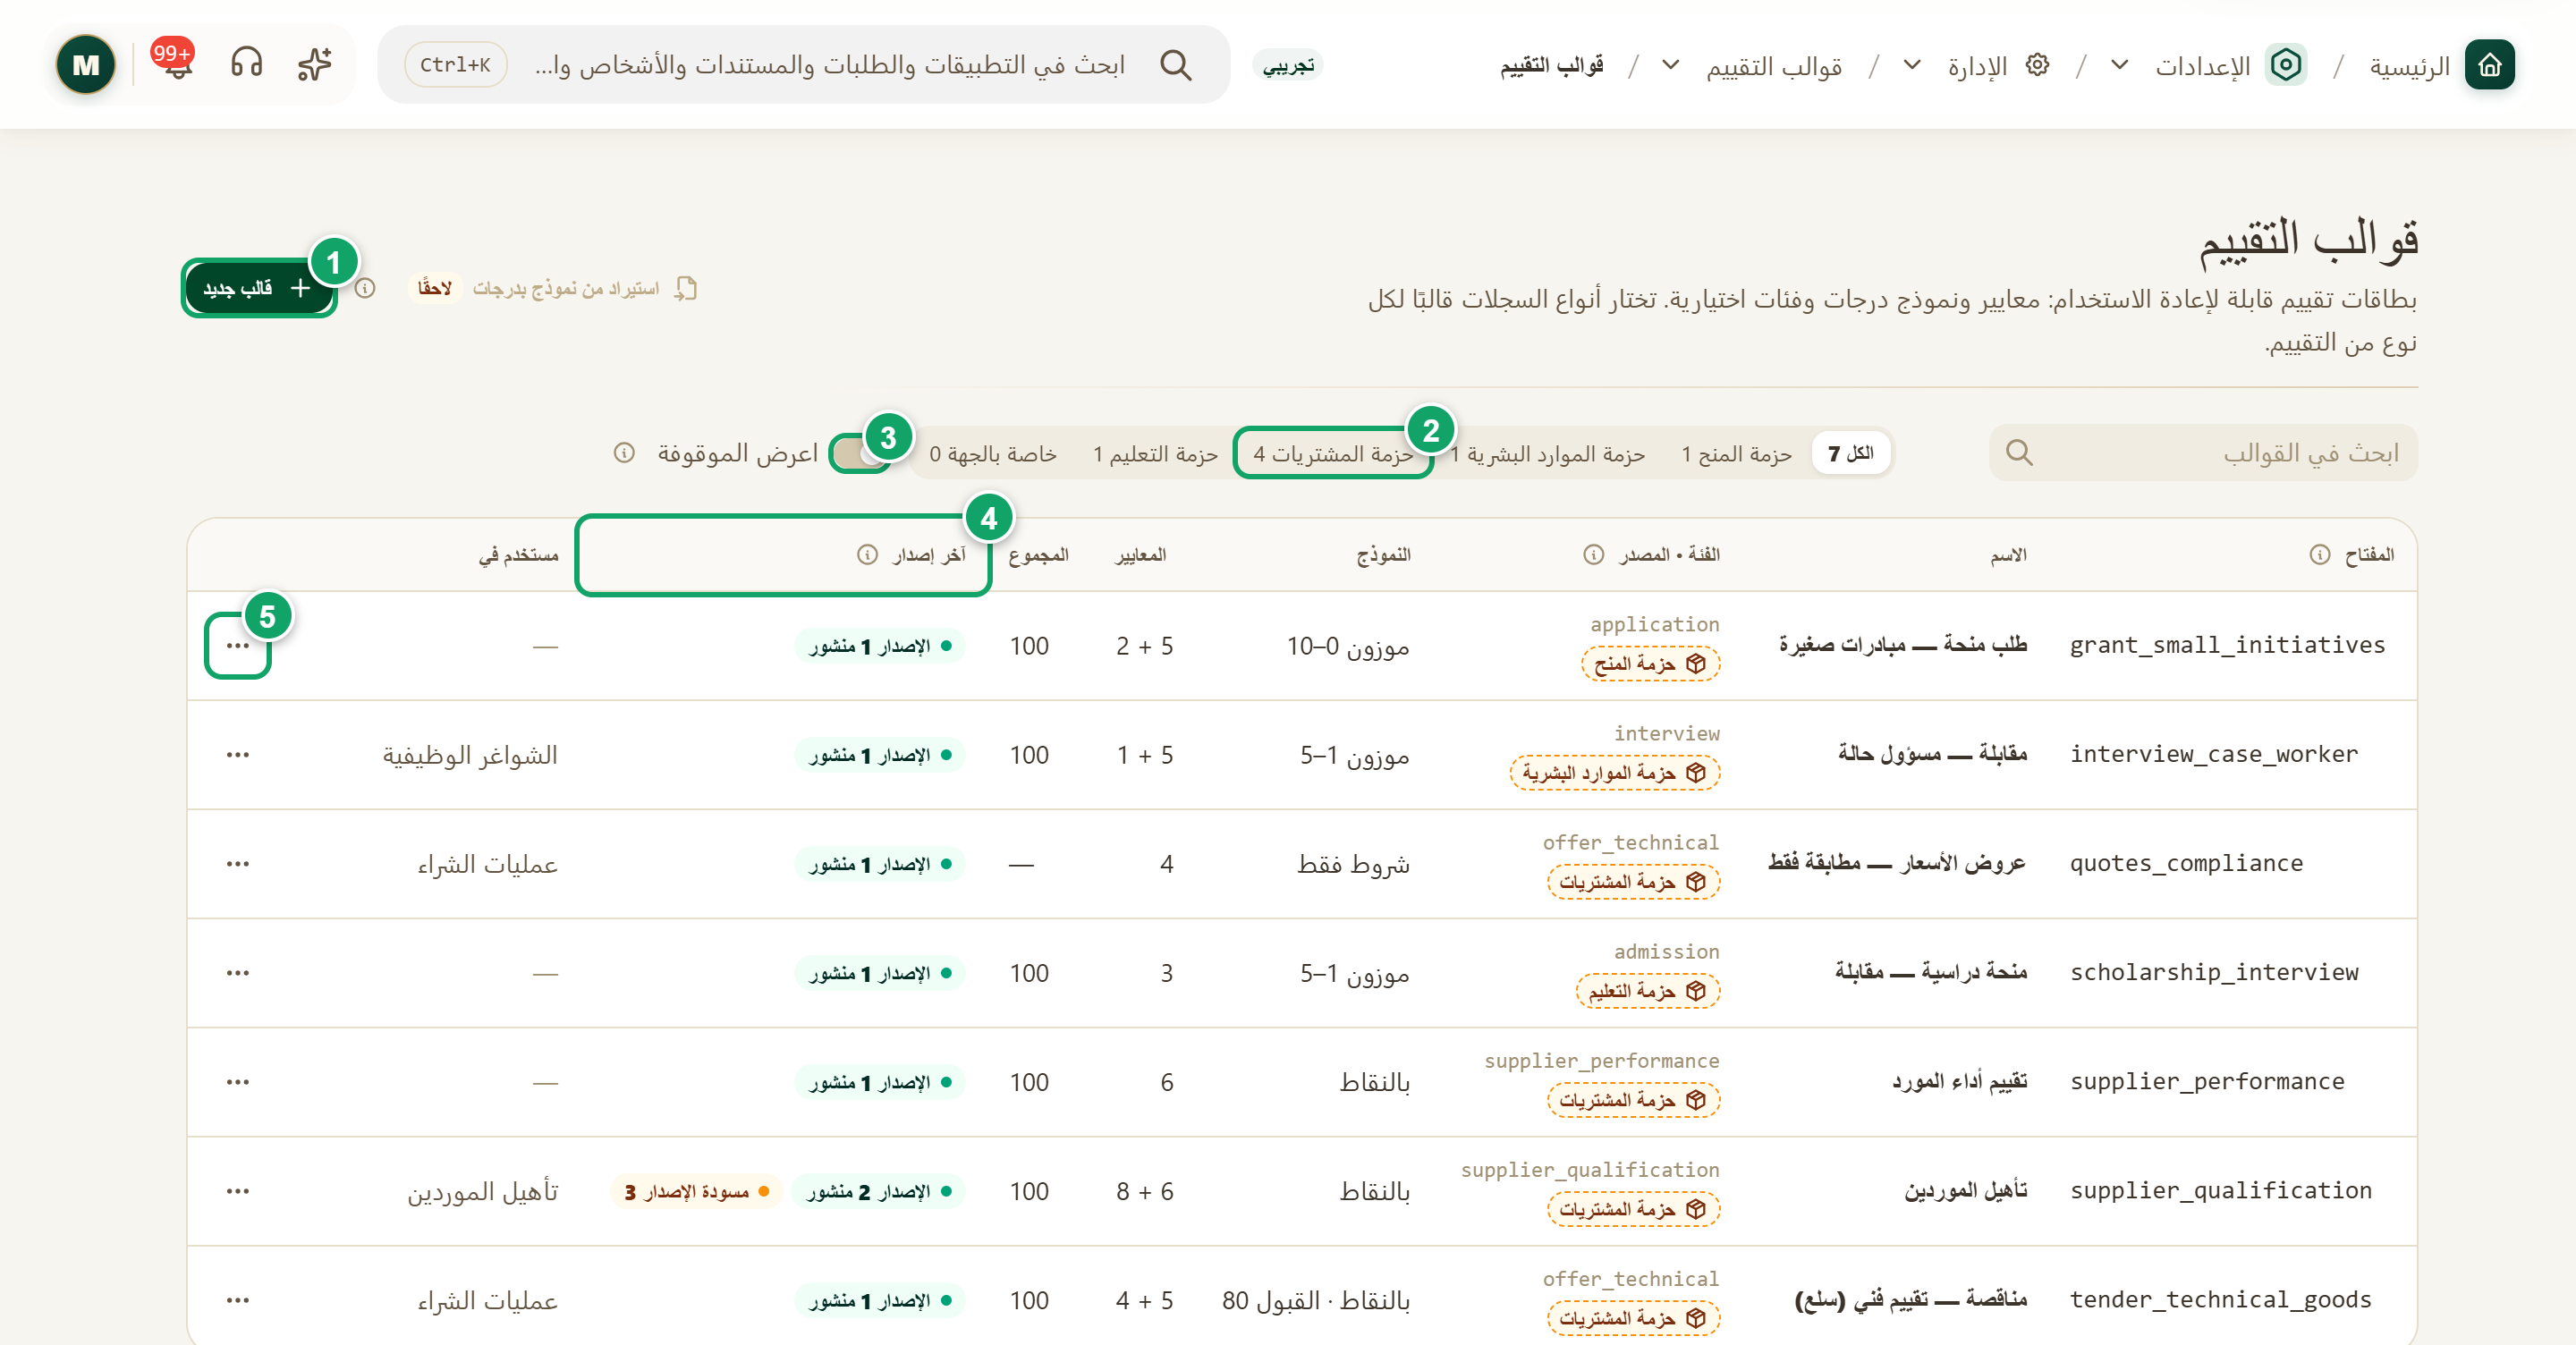
\includegraphics[width=0.95\linewidth,height=0.72\textheight,keepaspectratio]{figures/screens/ch08-evaluation-templates-ar.png}
\caption{مكتبة قوالب التقييم}
\label{fig:settings-evaluation-templates-screen}
\shotnote{تعرض المكتبة القوالب مع نموذج درجاتها وعدد معاييرها وآخر إصدار منها. والقوالب هنا قوالب جاهزة مثبتة في مؤسسة الاختبار، وخيار «استيراد من نموذج بدرجات» موسوم «لاحقًا» وغير متاح. ① «قالب جديد». ② تصفية بحسب مصدر القالب. ③ «اعرض الموقوفة». ④ «آخر إصدار». ⑤ قائمة القالب: نسخه أو عرض إصداراته أو «إيقاف».}
\end{figure}

\begin{figure}[H]
\centering
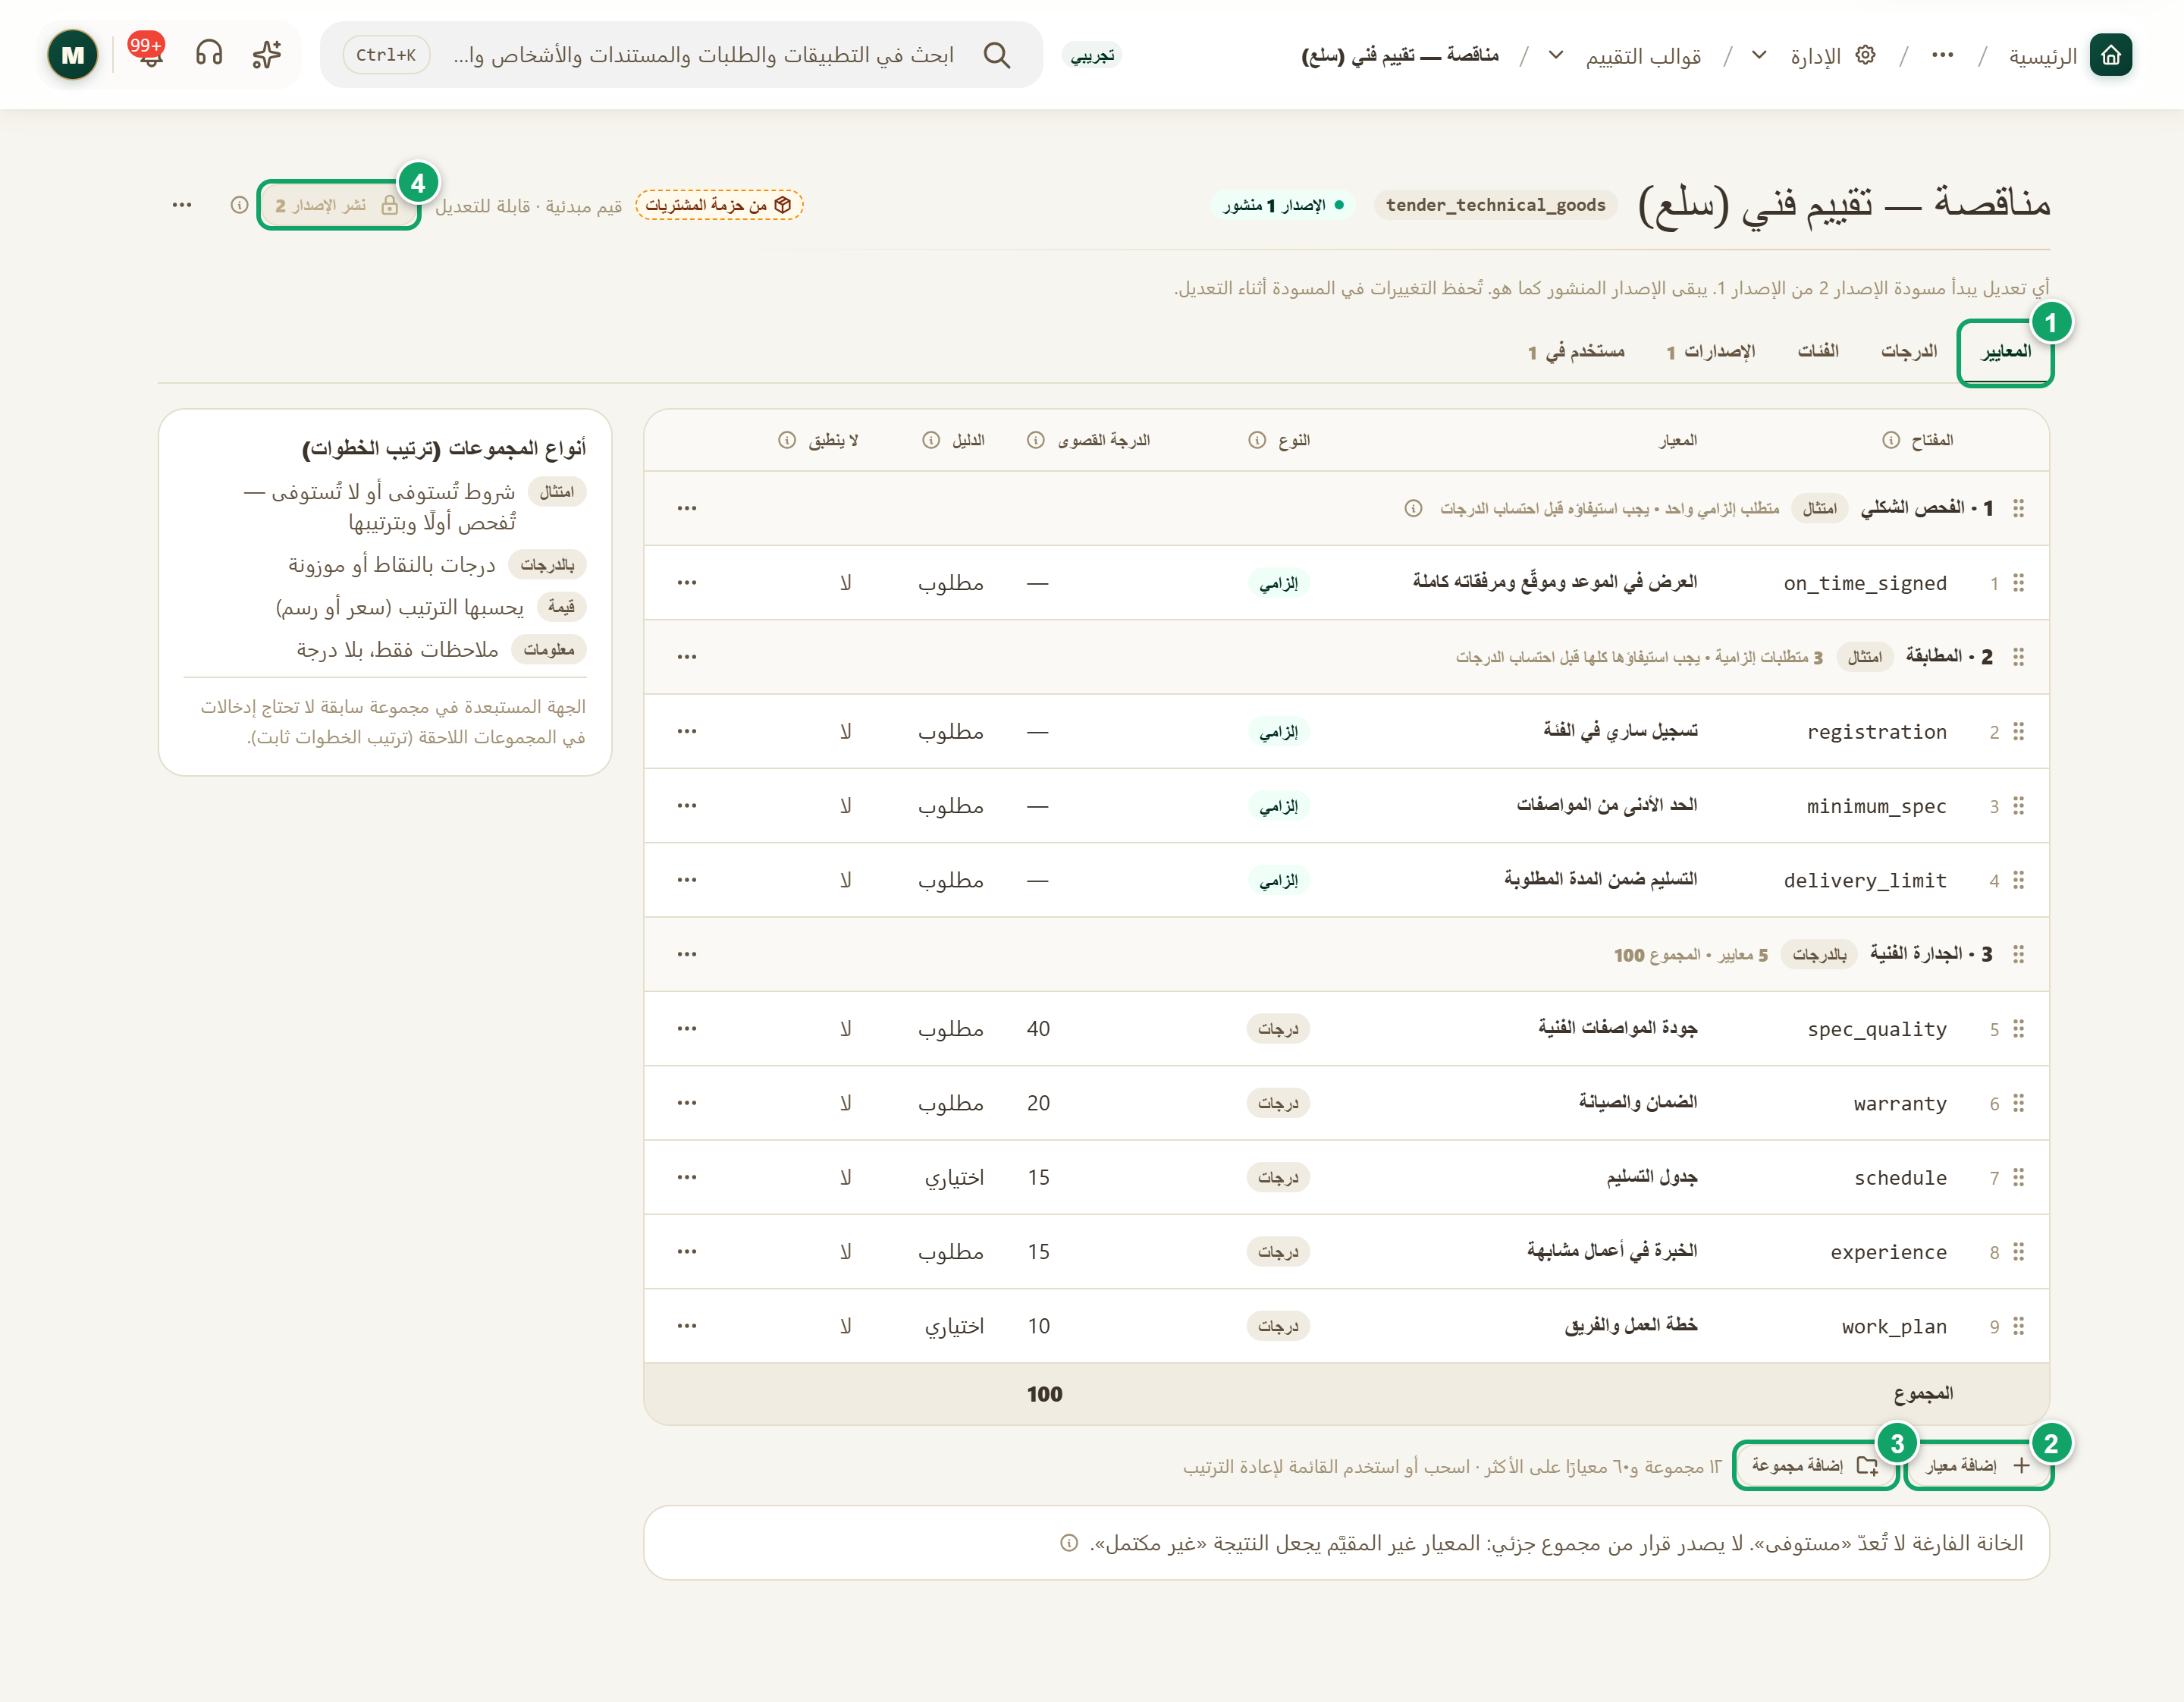
\includegraphics[width=0.95\linewidth,height=0.72\textheight,keepaspectratio]{figures/screens/ch08-evaluation-templates-criteria-ar.png}
\caption{تبويب المعايير}
\label{fig:settings-evaluation-templates-criteria-screen}
\shotnote{تُنظم المعايير في مجموعات تعمل بترتيبها؛ فمن يُستبعد في مجموعة «امتثال» لا يحتاج إلى إدخالات في المجموعات التالية. وأي تعديل هنا يبدأ مسودة، ويبقى الإصدار المنشور كما هو. ① «المعايير». ② «إضافة معيار». ③ «إضافة مجموعة». ④ «نشر الإصدار»: يبقى معطلاً ما دامت لا توجد مسودة.}
\end{figure}

\begin{figure}[H]
\centering
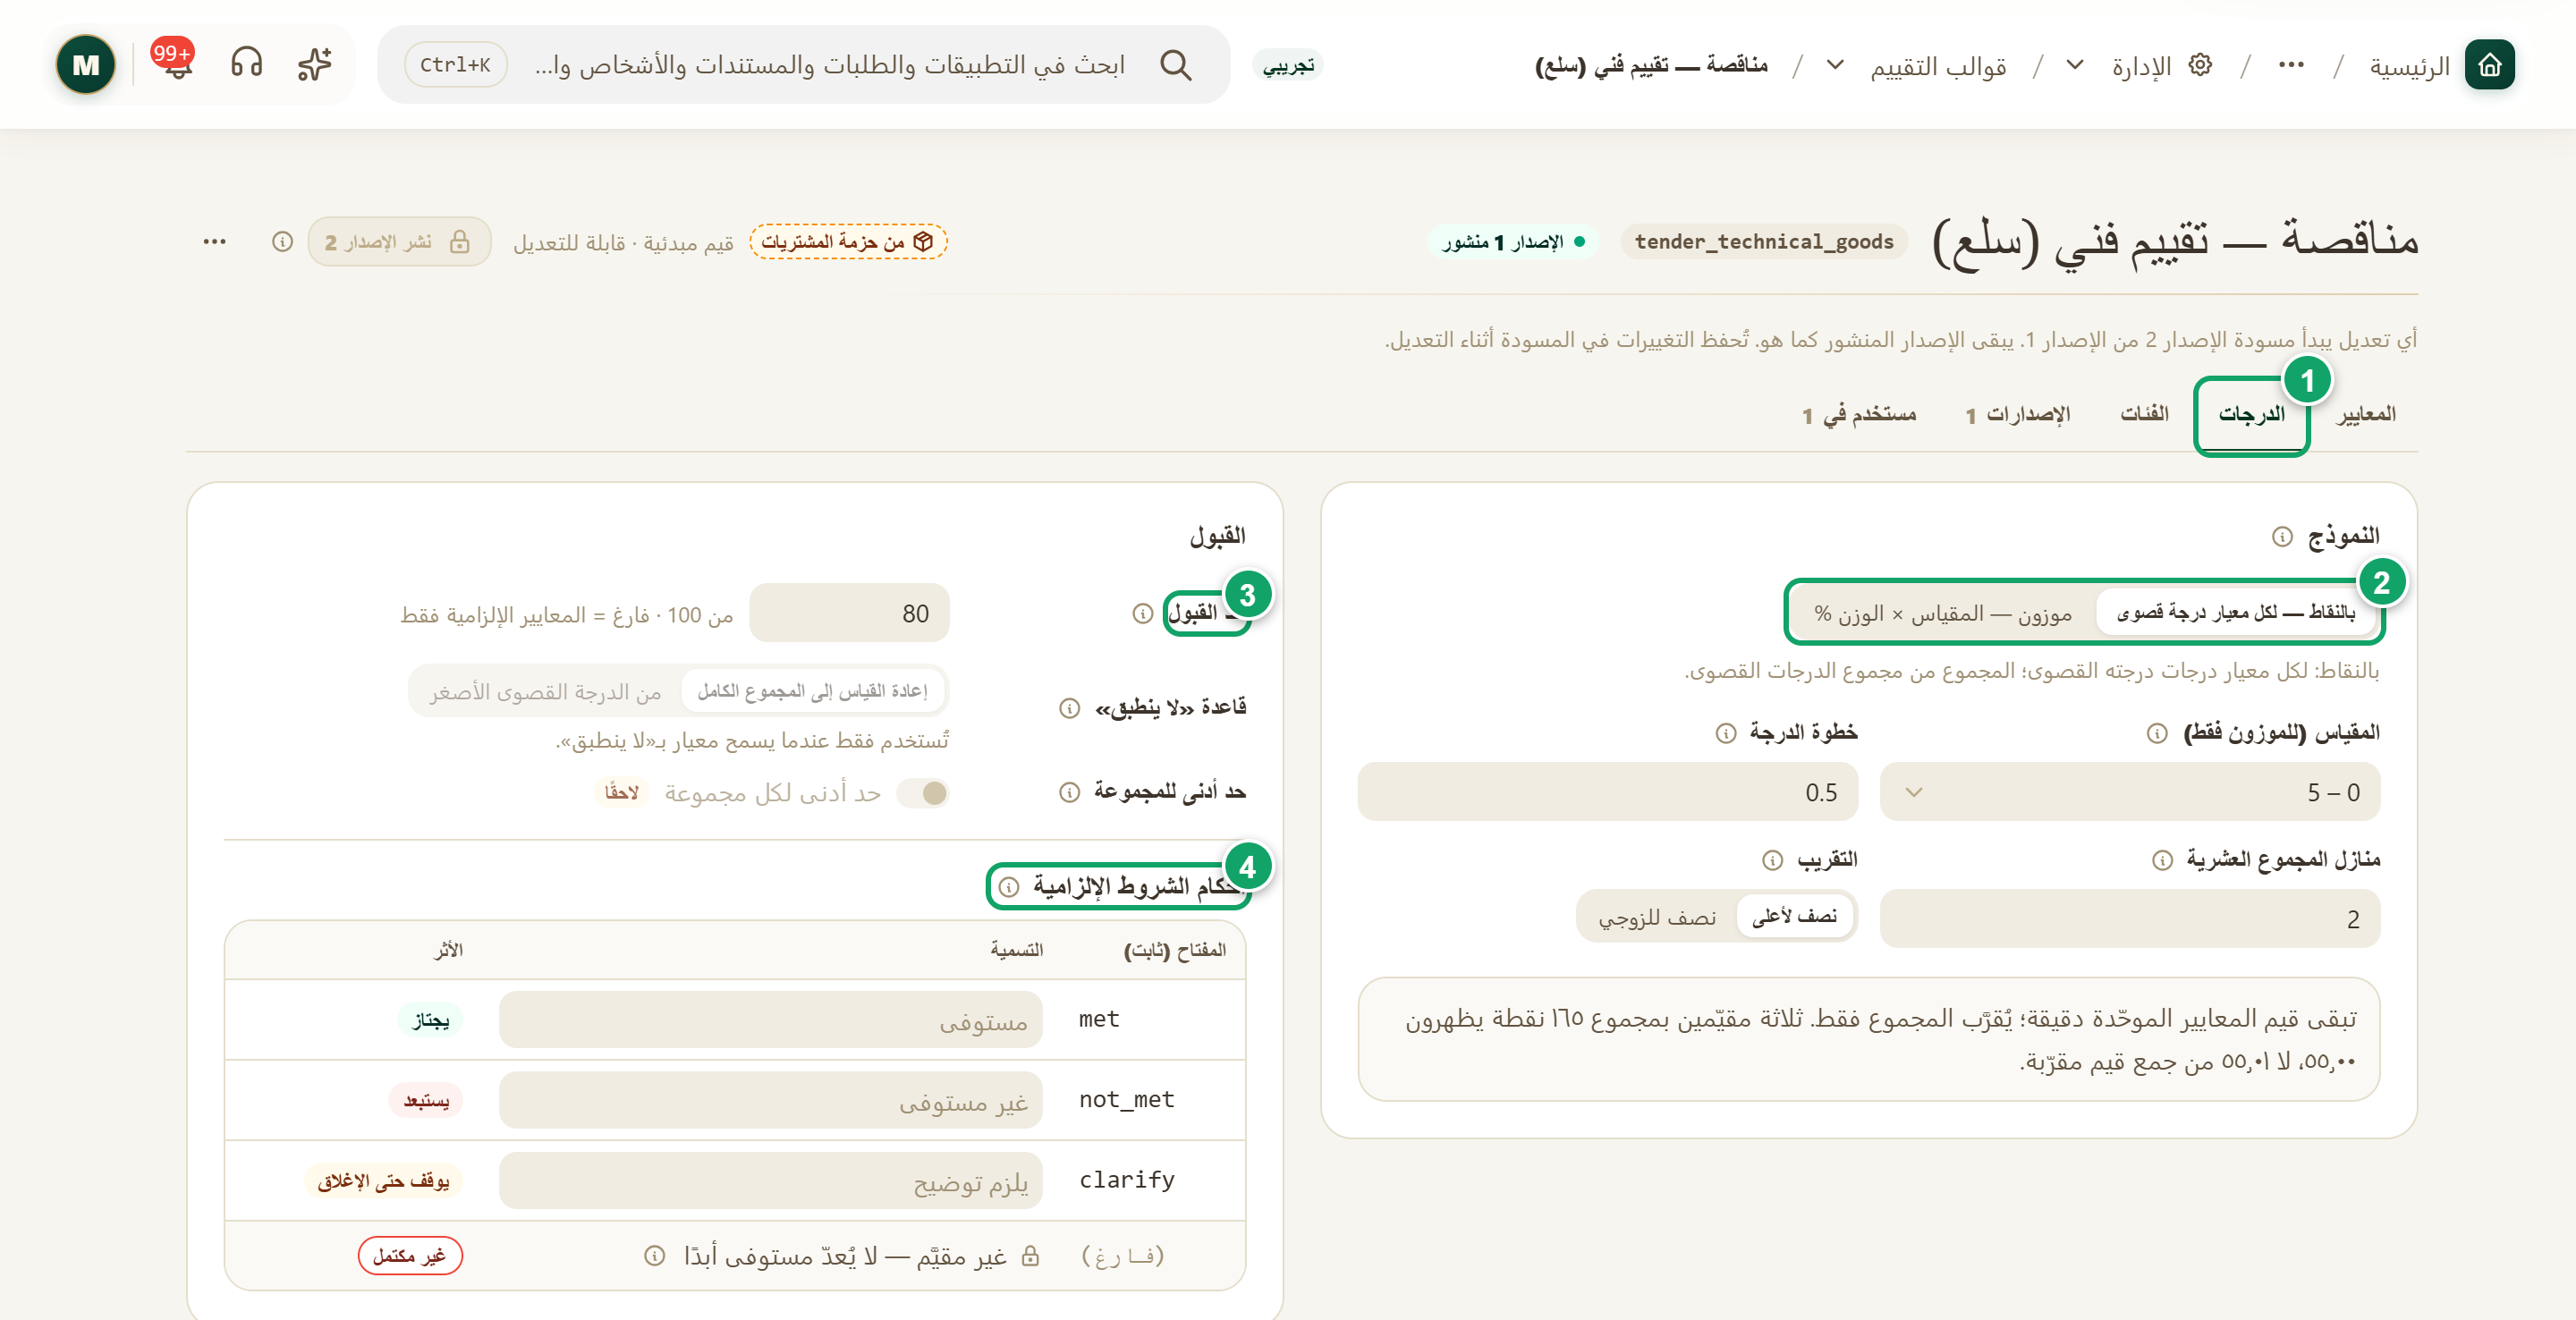
\includegraphics[width=0.95\linewidth,height=0.72\textheight,keepaspectratio]{figures/screens/ch08-evaluation-templates-scoring-ar.png}
\caption{تبويب الدرجات}
\label{fig:settings-evaluation-templates-scoring-screen}
\shotnote{يحدد التبويب طريقة حساب المجموع وشرط القبول. وتبقى قيم المعايير دقيقة ولا يُقرَّب إلا المجموع، فلا ينشأ فرق من جمع قيم مقرّبة. ① «الدرجات». ② «نموذج الدرجات»: نقاط لكل معيار أو سلم مع أوزان. ③ «حد القبول»: إذا تُرك فارغاً اكتُفي بالشروط الإلزامية. ④ «أحكام الشروط الإلزامية»: الخانة الفارغة لا تُعد مستوفاة أبداً.}
\end{figure}

\begin{figure}[H]
\centering
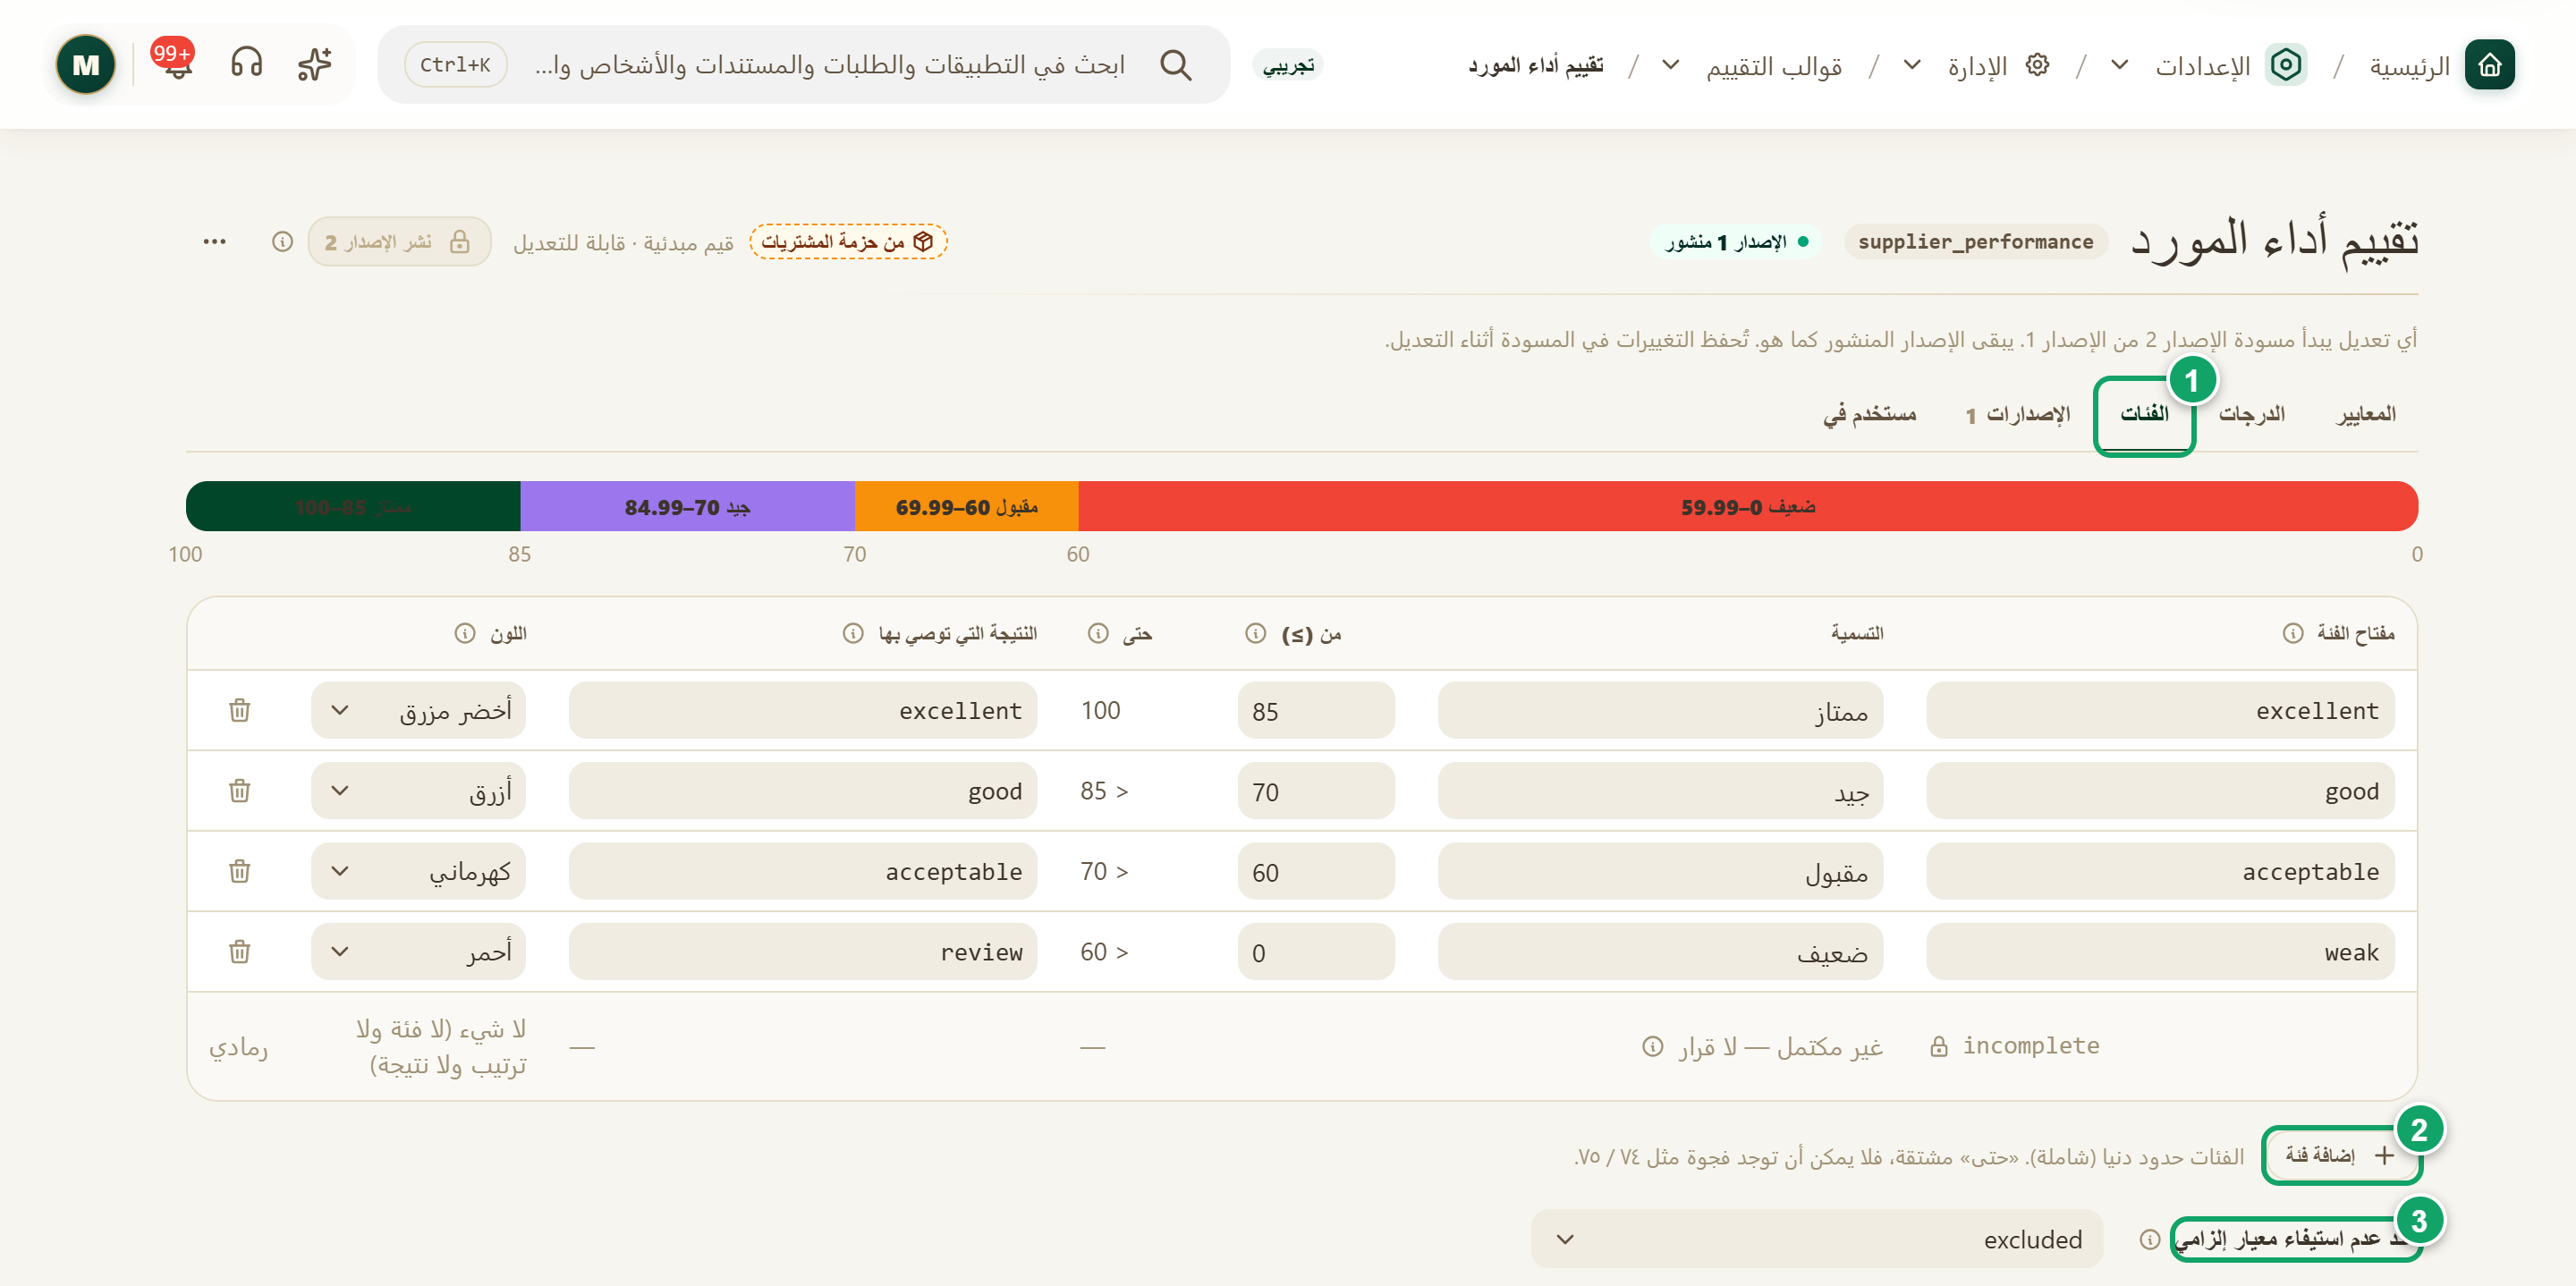
\includegraphics[width=0.95\linewidth,height=0.72\textheight,keepaspectratio]{figures/screens/ch08-evaluation-templates-bands-ar.png}
\caption{تبويب الفئات}
\label{fig:settings-evaluation-templates-bands-screen}
\shotnote{تحوّل الفئات المجموع إلى نتيجة مفهومة، مثل مقبول أو ضعيف. وتحدد كل فئة حدها الأدنى فقط، فيُحسب الحد الأعلى تلقائياً ولا تنشأ فجوة بين فئتين. ① «الفئات». ② «إضافة فئة». ③ النتيجة عند عدم استيفاء معيار إلزامي.}
\end{figure}

\begin{table}[H]
\centering
\caption{ماذا تسجل في القالب؟}
\label{tab:settings-evaluation-templates-fields}
\begin{tabularx}{\linewidth}{R{4.2cm} Y}
\rcHeaderRow
\thh{الجزء} & \thh{ماذا تسجل فيه؟}\\
القالب الجديد & «المفتاح»، و«الاسم»، و«الفئة»، و«ابدأ من»: قالب فارغ أو قالب جاهز من حزمة أو نسخة من قالب آخر.\\
«المعايير» & مجموعات من أربعة أنواع: «امتثال» و«بالدرجات» و«قيمة» و«معلومات». ولكل معيار مفتاحه وتسميته ونوعه ودرجته القصوى أو وزنه، و«الدليل»، وإرشادات التقييم، وخيار «لا ينطبق».\\
«الدرجات» & «نموذج الدرجات»، والسلم، وخطوة الدرجة، ومنازل المجموع، والتقريب، و«حد القبول»، و«أحكام الشروط الإلزامية».\\
«الفئات» & مفتاح الفئة وتسميتها وحدها الأدنى والنتيجة التي توصي بها ولونها.\\
«الإصدارات» & الإصدارات المنشورة مع تاريخها وناشرها وملاحظتها وبصمتها.\\
«مستخدم في» & أنواع السجلات التي تستخدم القالب وتقييماتها المفتوحة. ويختار نوع السجل القالب من أداة البناء.\\
\end{tabularx}
\end{table}

\begin{enumerate}
\item افتح «الإعدادات» ثم «قوالب التقييم»، واضغط «قالب جديد».
\item اكتب «المفتاح» و«الاسم»، واختر نقطة البداية من «ابدأ من»، ثم اضغط «إنشاء مسودة».
\item أضف المجموعات والمعايير، ثم اضبط «الدرجات» و«الفئات». تُحفظ التغييرات في المسودة تلقائياً.
\item عالج المشكلات المعروضة، ثم اضغط «نشر الإصدار» واكتب ملاحظة تبيّن سببه.
\item إذا لم تعد تحتاج إلى قالب، فافتح قائمته واضغط «إيقاف»؛ إذ لا يوجد حذف للقوالب.
\end{enumerate}

\textbf{تحقق:} يظهر القالب في المكتبة بشارة الإصدار المنشور، ويمكن لنوع السجل اختياره. وعند نشر إصدار جديد تبقى التقييمات المفتوحة على إصدارها المثبت، ويسري الجديد على التقييمات الجديدة فقط. وإذا بقي زر النشر معطلاً، فراجع المشكلات المعروضة؛ فمجموع الأوزان مثلاً يجب أن يساوي 100.

\section{المتابعة}
\label{sec:settings-feature-followup}

تضبط هذه الصفحة الكلمات المشتركة التي تستخدمها لوحات المتابعة لتفسير التأخير. فـ«سبب التعطل» يقول لماذا ينتظر السجل في مرحلته، و«نوع العائق» يربط سجلاً بآخر يمنعه من التقدم، و«التدخل» قرار يُطلب من جهة أعلى لإنهاء التعطل. تعمل اللوحات دون أسباب أيضاً، لكنها تعرض الصفوف المتأخرة عندها «غير مبرَّرة». ويستطيع المخوَّلون قراءة الصفحة، أما تعديلها فيحتاج إلى صلاحية «ضبط المتابعة».

\begin{rcnote}[مثال: شركة الأفق]
يضغط مسؤول النظام «سبب جديد» عند ② ويضيف سبب «بانتظار موافقة المورد». وعندما تتأخر زيارة فرع حلب، تختار سارة الخطيب هذا السبب، فتظهر المدة ضمن هذا السبب في اللوحة بدلاً من تأخير غير مفسَّر.
\end{rcnote}

\begin{figure}[H]
\centering
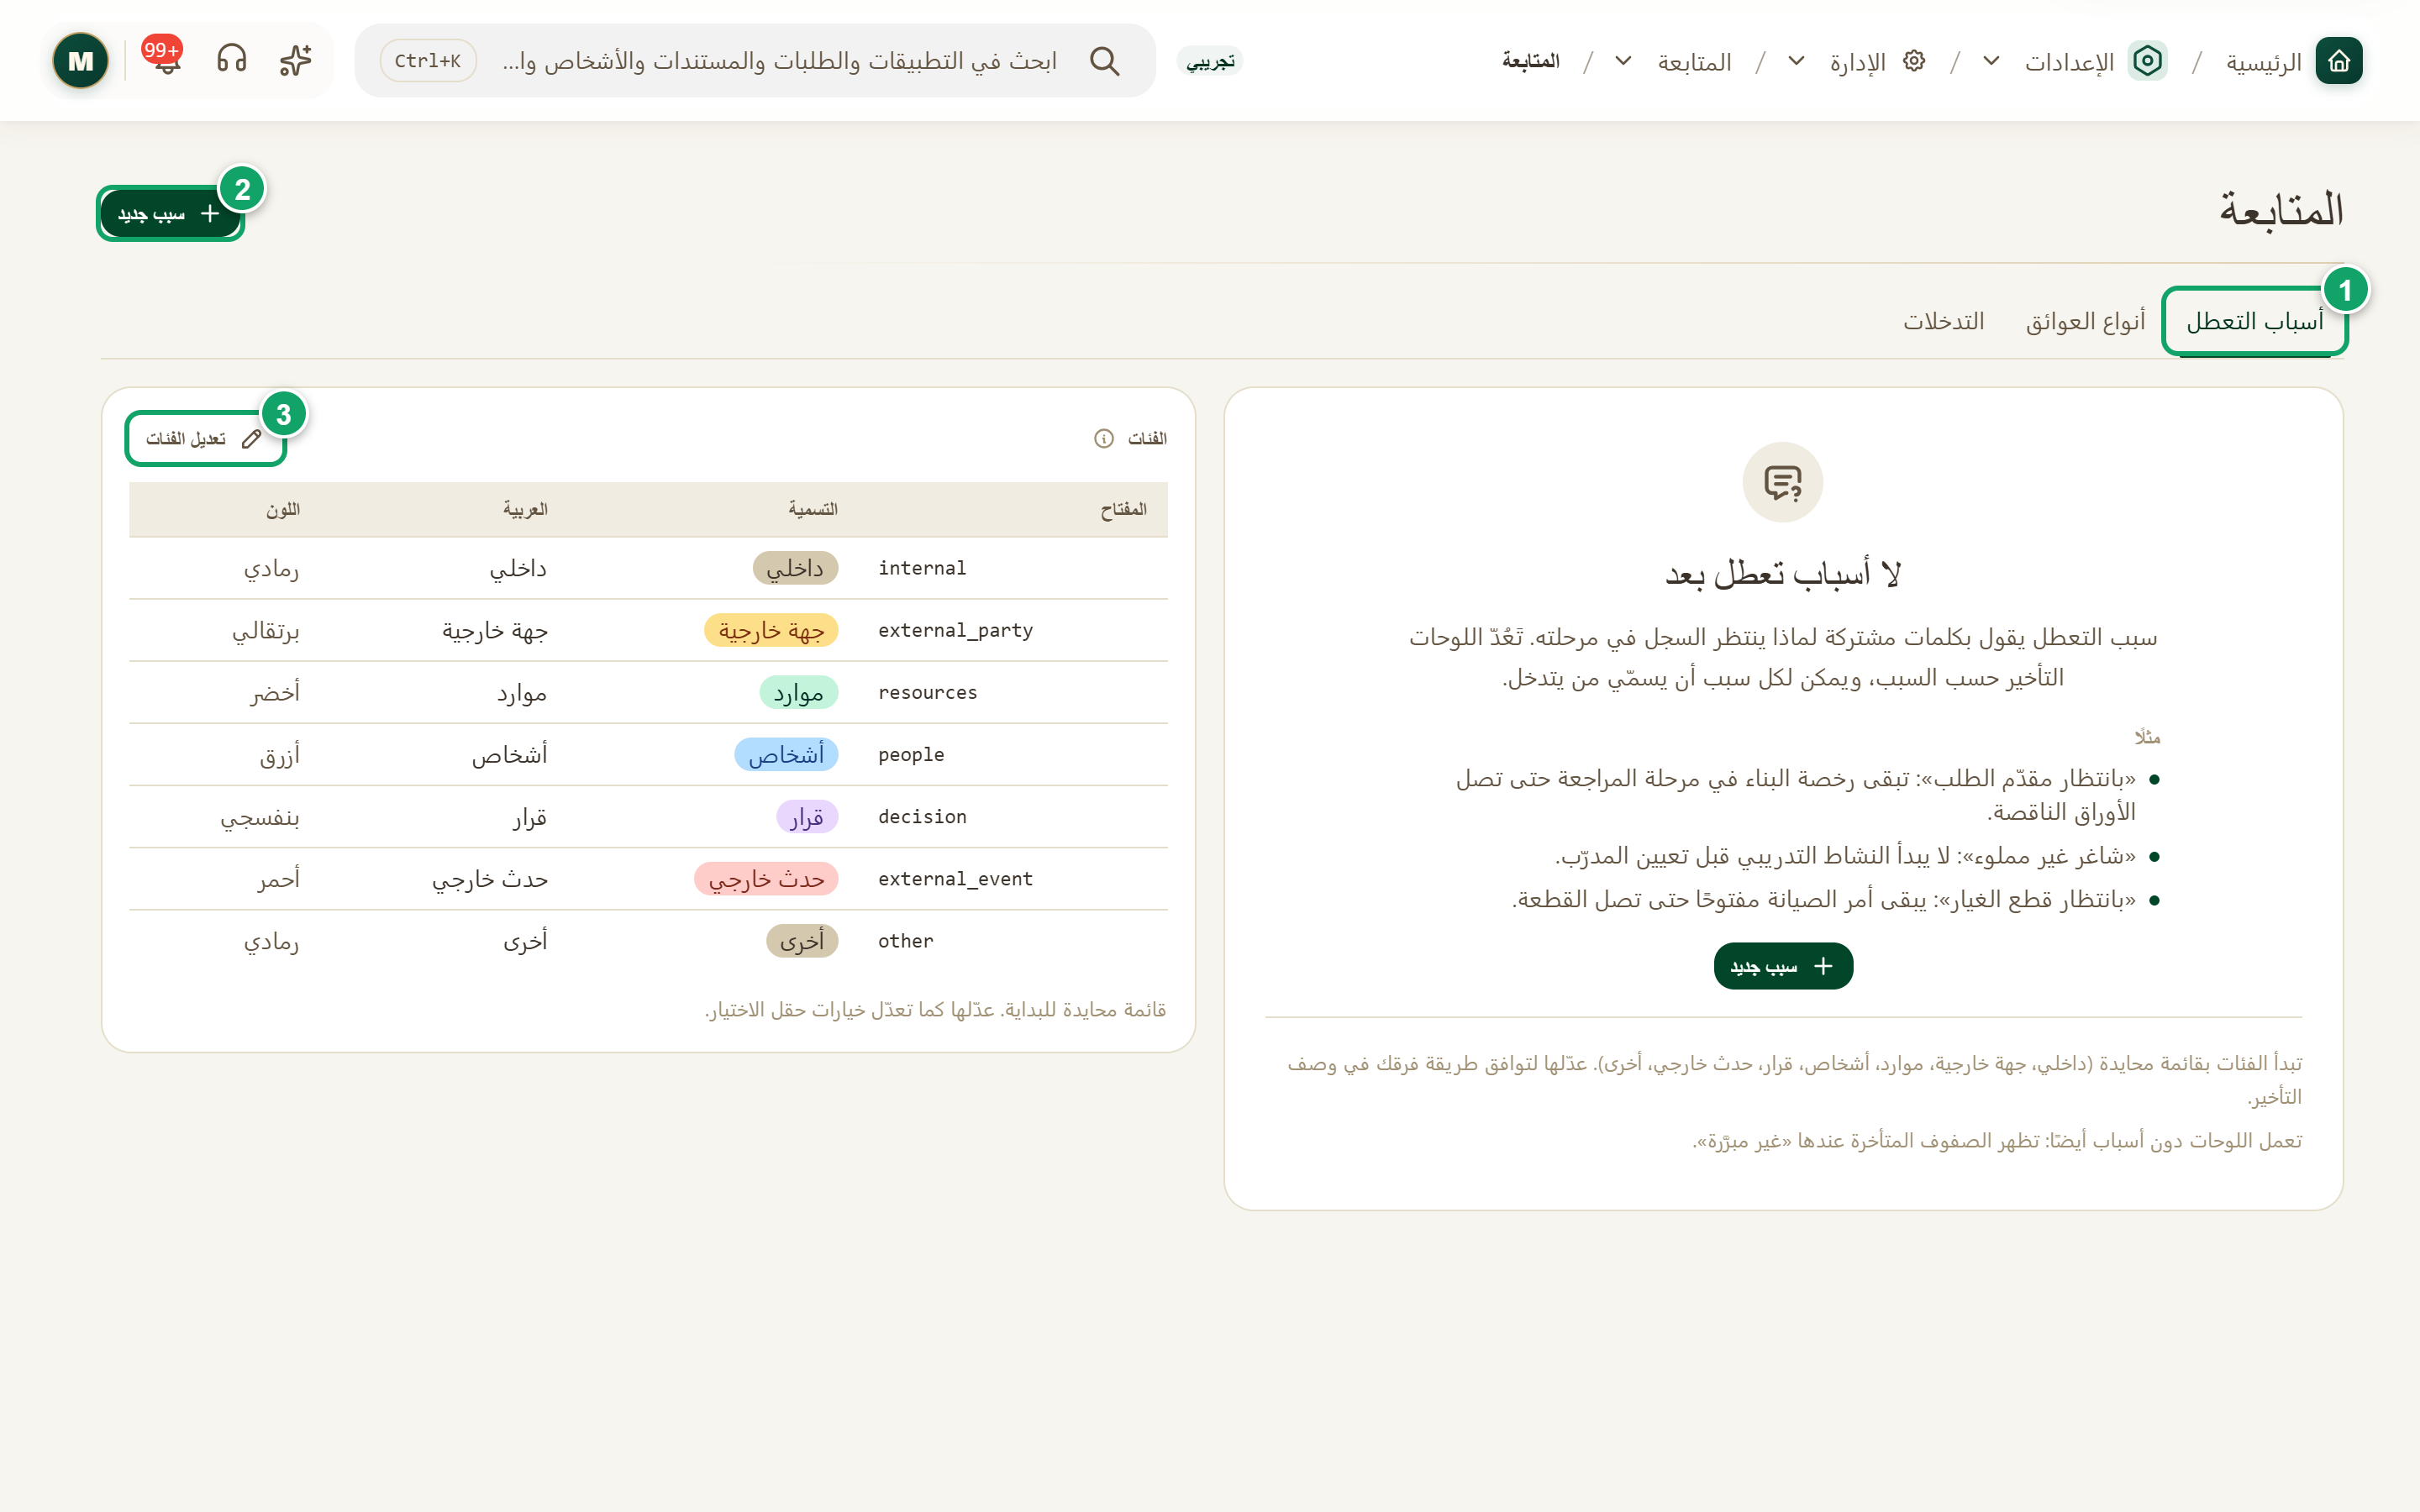
\includegraphics[width=0.95\linewidth,height=0.72\textheight,keepaspectratio]{figures/screens/ch08-followup-ar.png}
\caption{أسباب التعطل والفئات}
\label{fig:settings-followup-screen}
\shotnote{تعرض الصورة الحالة الفارغة في مؤسسة الاختبار، إذ لا تضم أسباباً بعد، مع قائمة الفئات التي تبدأ بها كل مؤسسة. وتجمع الفئات الأسباب لتحسب اللوحات التأخير بحسب مصدره. ① «أسباب التعطل». ② «سبب جديد». ③ «تعديل الفئات».}
\end{figure}

\begin{figure}[H]
\centering
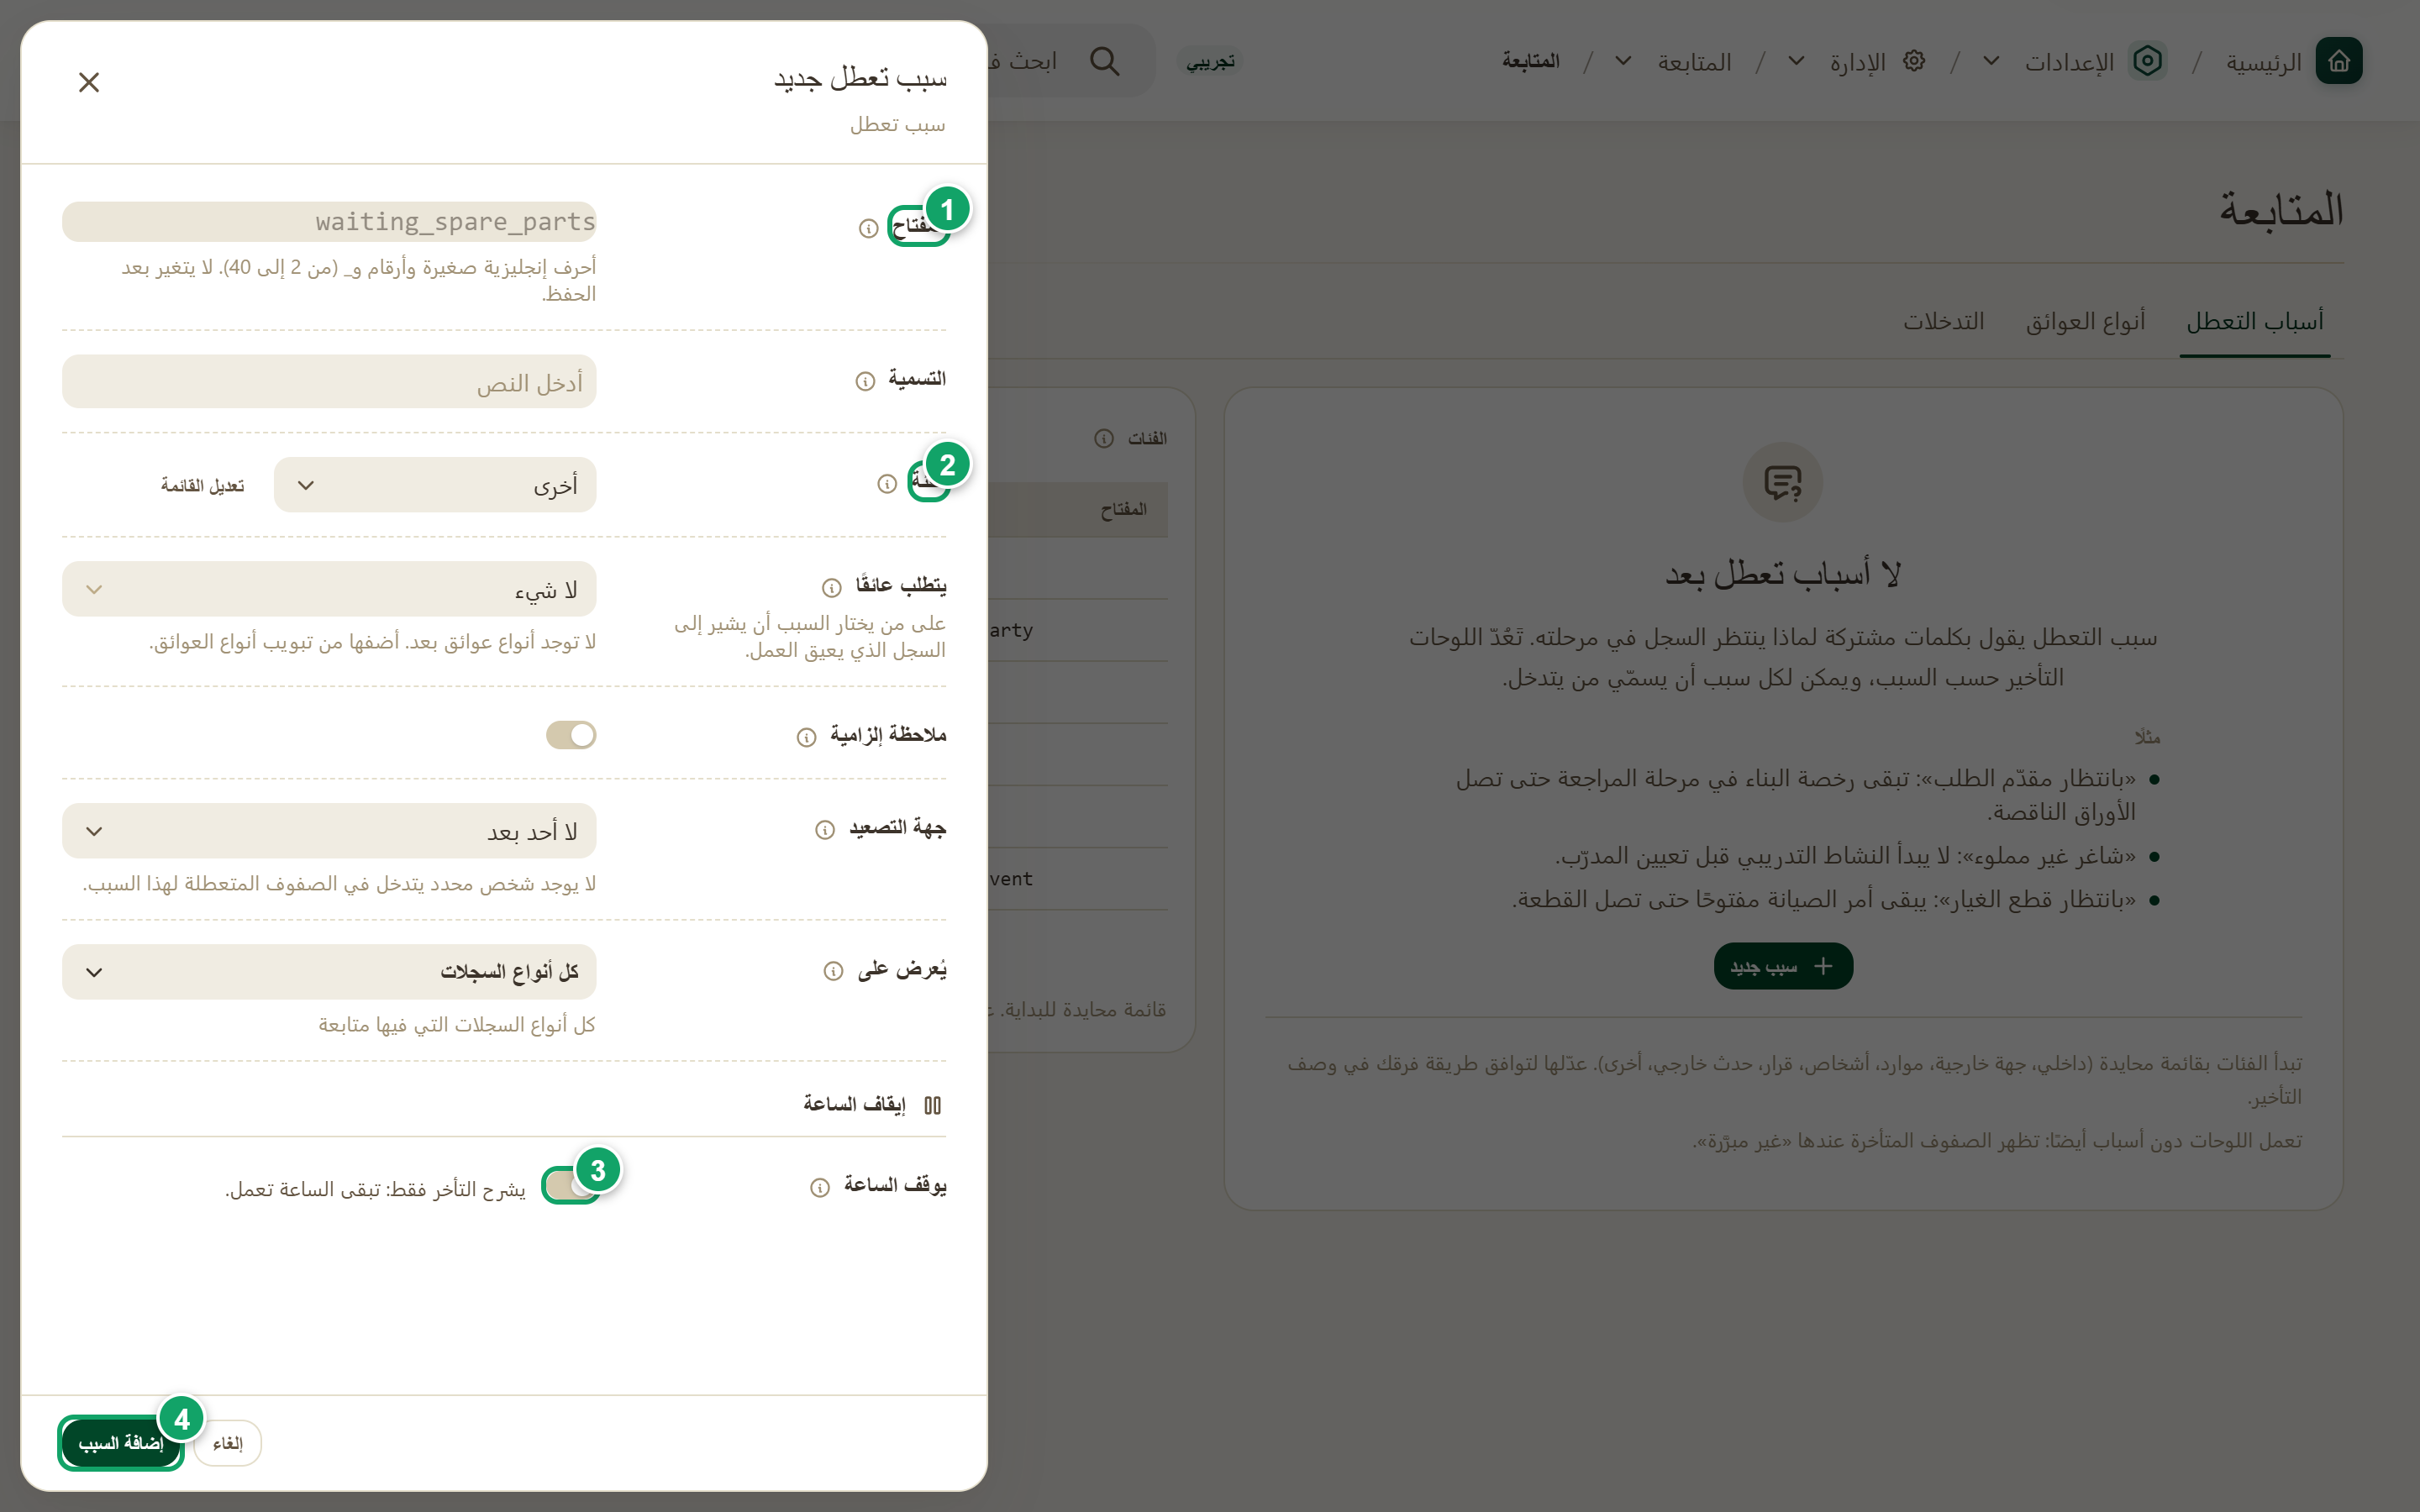
\includegraphics[width=0.95\linewidth,height=0.72\textheight,keepaspectratio]{figures/screens/ch08-followup-reason-ar.png}
\caption{نافذة سبب تعطل جديد}
\label{fig:settings-followup-reason-screen}
\shotnote{تحدد النافذة معنى السبب وأثره في عمل الفريق. وأهم قرار فيها هو إيقاف الساعة؛ فهو يميز التأخير الذي يُفسَّر فقط من الانتظار الذي لا يُحتسب على المرحلة. ① «المفتاح»: يُملأ من التسمية ولا يتغير بعد الحفظ. ② «الفئة». ③ «يوقف الساعة»: عند تفعيله تظهر خيارات الاستئناف والحدود. ④ «إضافة السبب».}
\end{figure}

\begin{figure}[H]
\centering
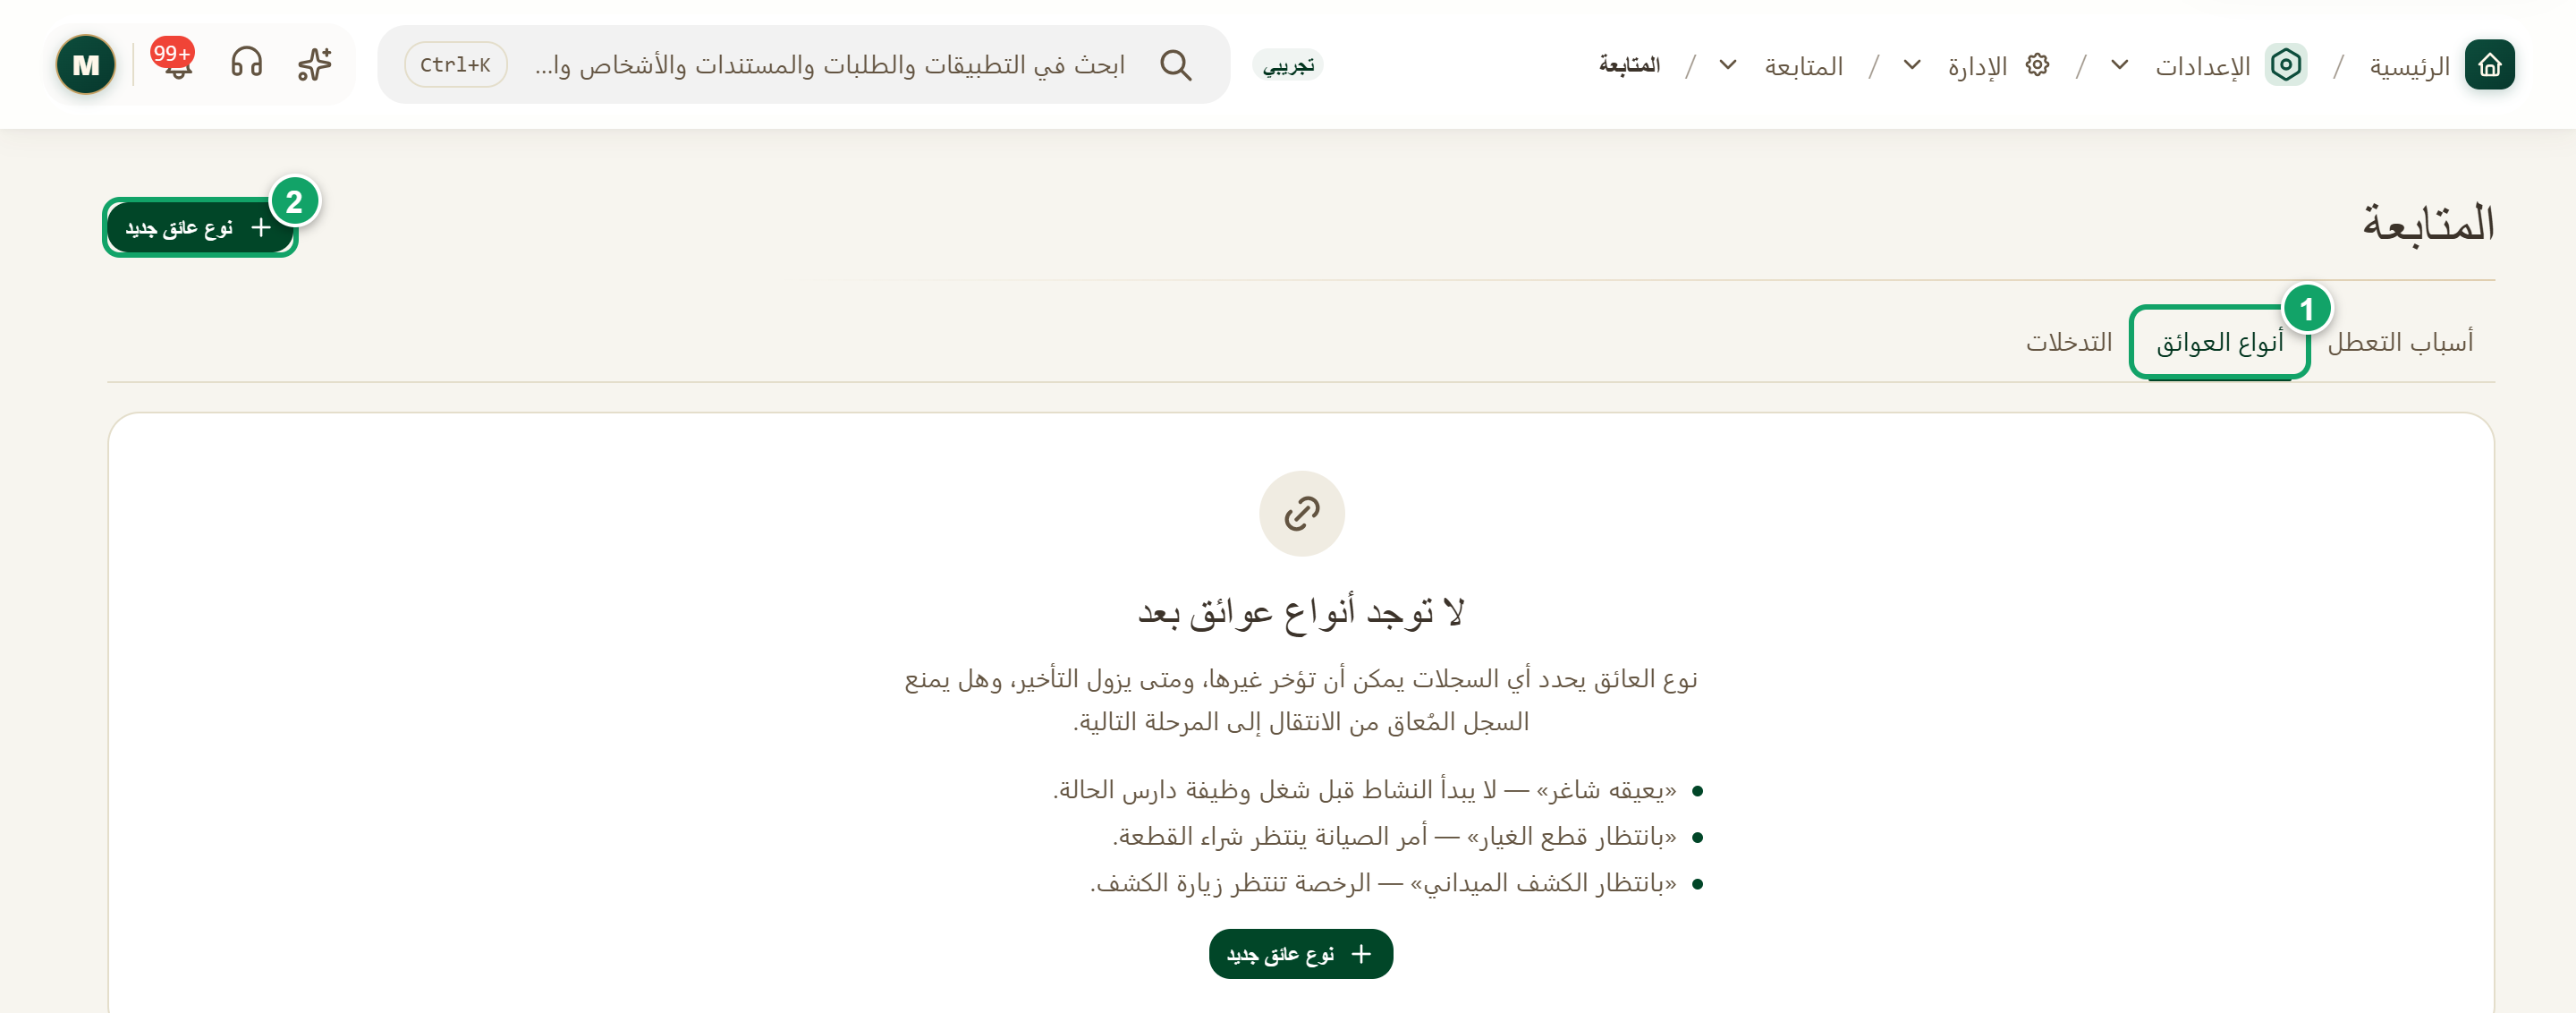
\includegraphics[width=0.95\linewidth,height=0.72\textheight,keepaspectratio]{figures/screens/ch08-followup-blockers-ar.png}
\caption{أنواع العوائق}
\label{fig:settings-followup-blockers-screen}
\shotnote{يحدد نوع العائق السجلات التي يمكن أن تعيق غيرها، ومتى يزول العائق، وهل يمنع السجل من التقدم. والتبويب فارغ في مؤسسة الاختبار، لذلك تعرض الصورة الشرح والأمثلة التي يقدمها النظام. ① «أنواع العوائق». ② «نوع عائق جديد».}
\end{figure}

\begin{figure}[H]
\centering
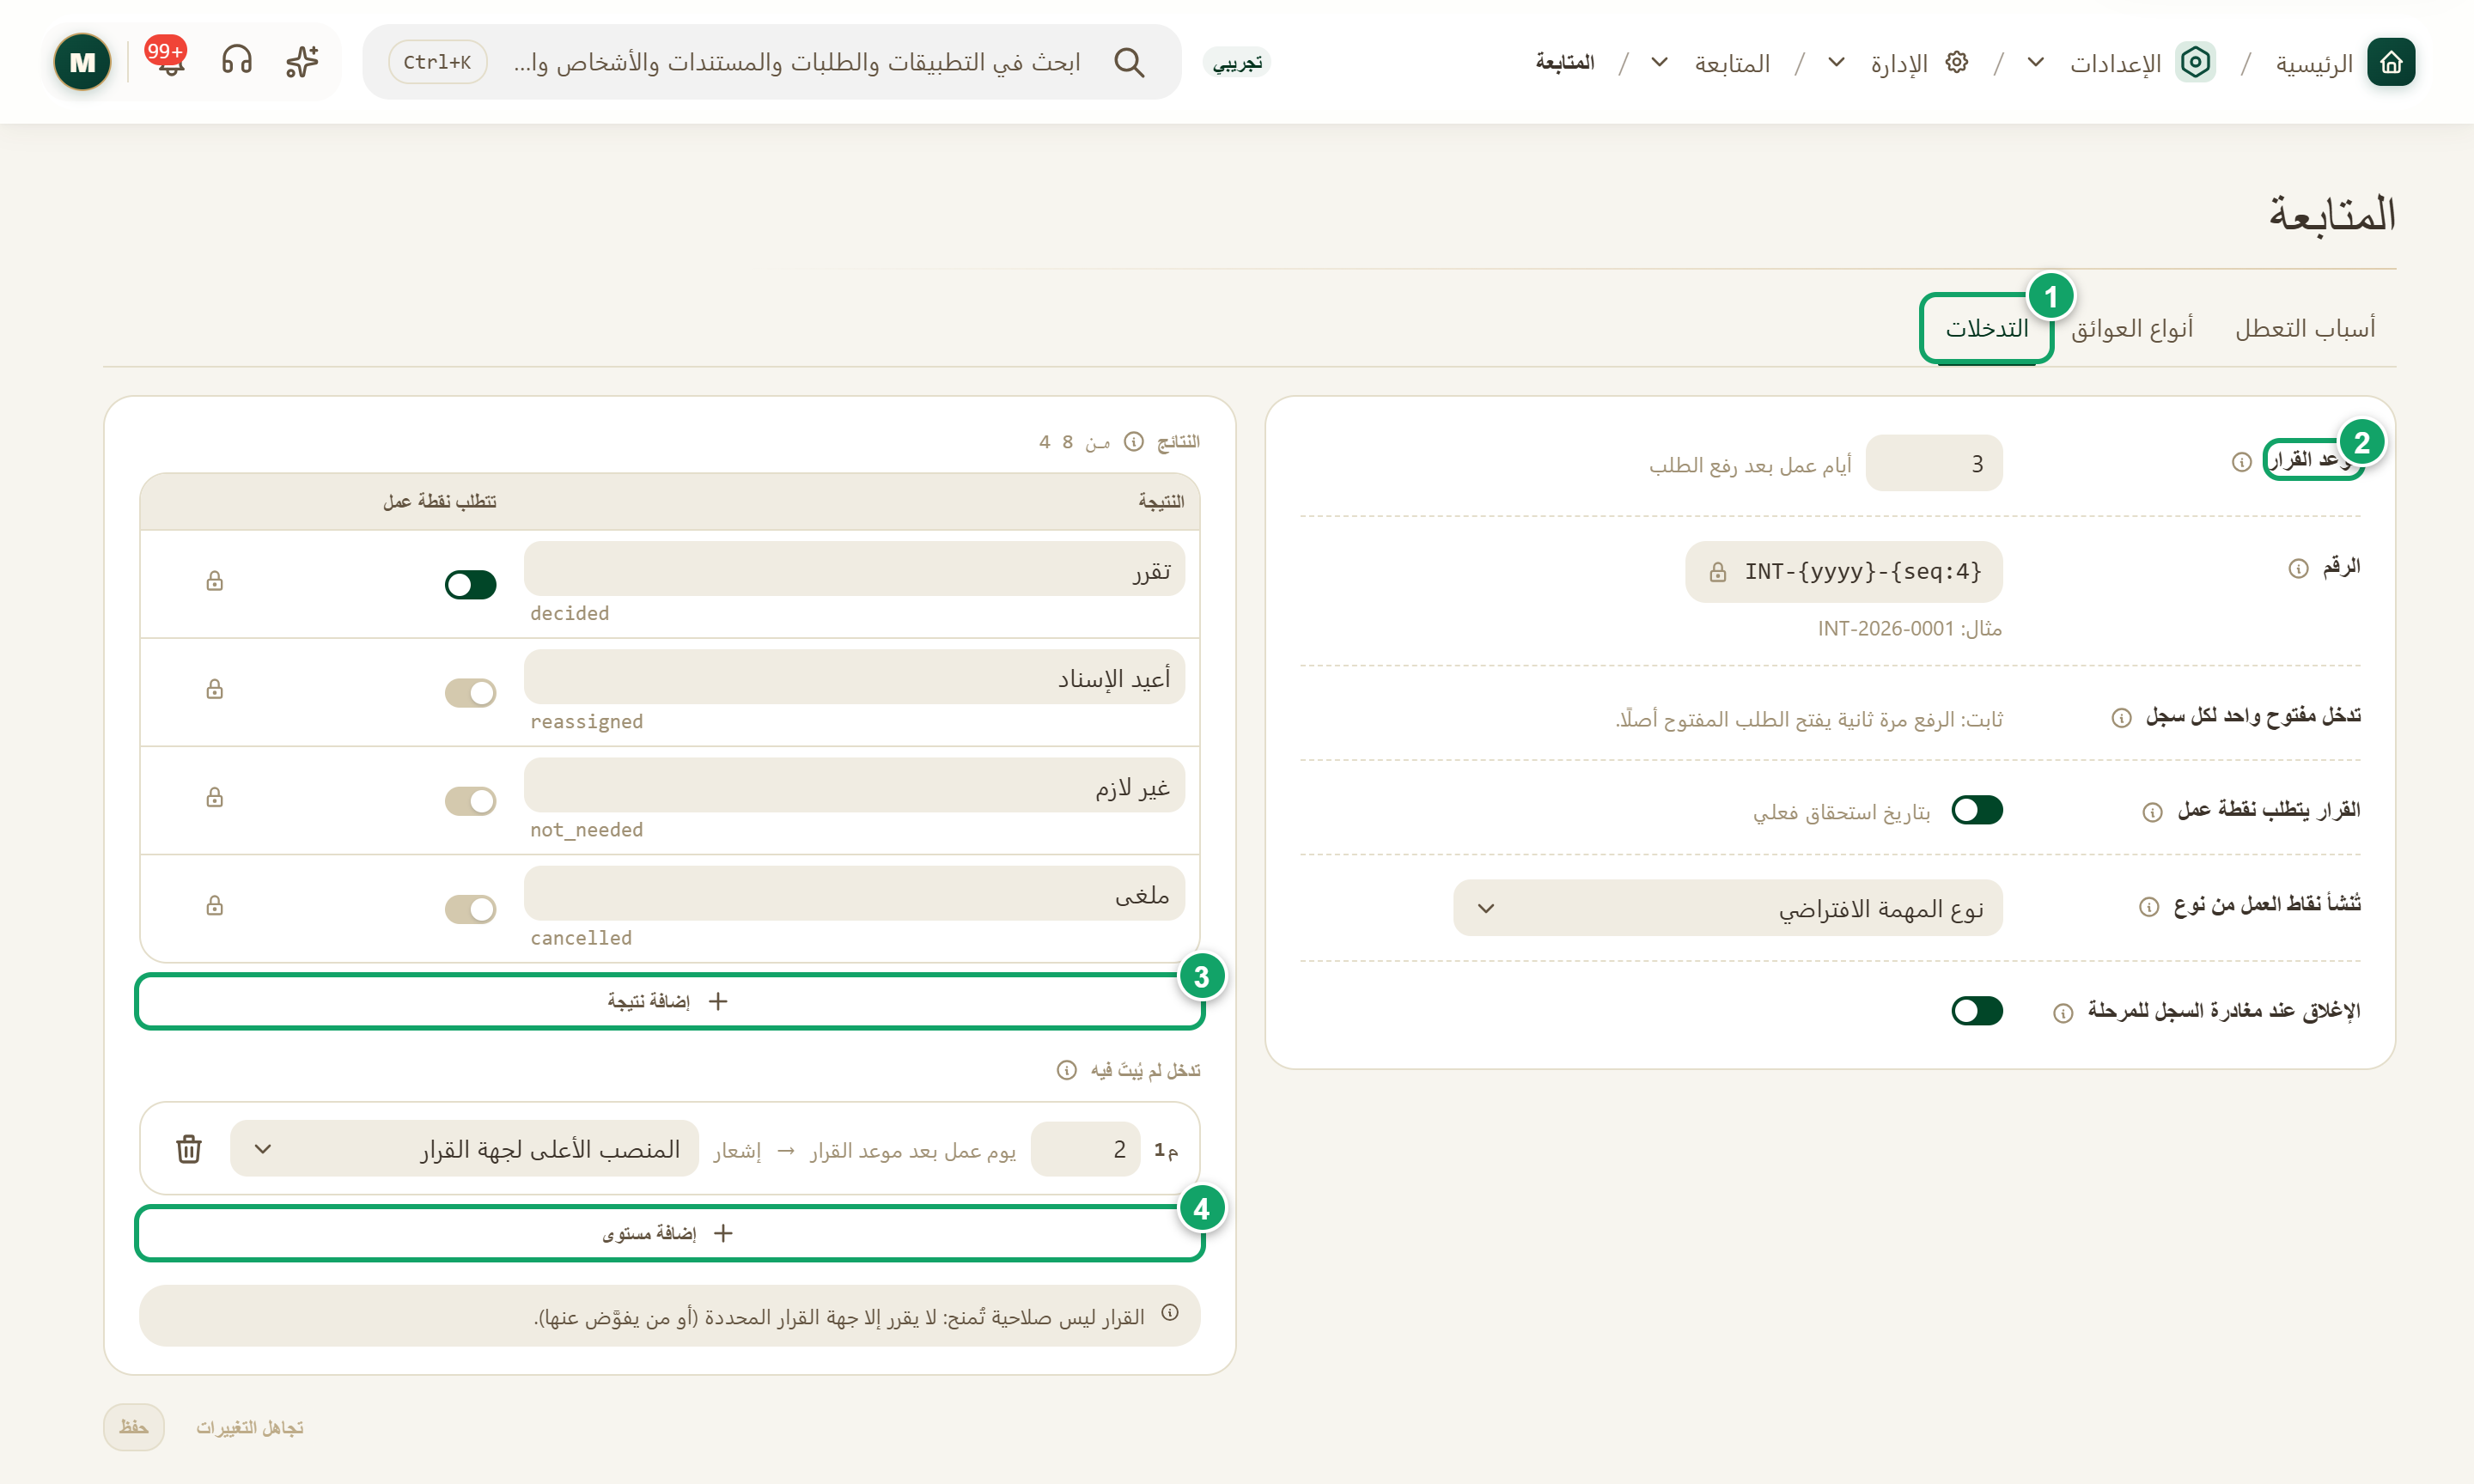
\includegraphics[width=0.95\linewidth,height=0.72\textheight,keepaspectratio]{figures/screens/ch08-followup-interventions-ar.png}
\caption{إعدادات التدخلات}
\label{fig:settings-followup-interventions-screen}
\shotnote{يحدد التبويب مهلة قرار التدخل، والنتائج التي يمكن تسجيلها، ومن يُبلَّغ إذا لم يُبتّ فيه. والقرار نفسه ليس صلاحية تُمنح؛ فلا تقرر إلا الجهة المحددة أو من تفوضه. ① «التدخلات». ② «موعد القرار». ③ «إضافة نتيجة». ④ «إضافة مستوى»: يضيف مرحلة تنبيه بعد موعد القرار.}
\end{figure}

\begin{table}[H]
\centering
\caption{ماذا تسجل في كل تبويب؟}
\label{tab:settings-followup-fields}
\begin{tabularx}{\linewidth}{R{4.2cm} Y}
\rcHeaderRow
\thh{التبويب} & \thh{ماذا تسجل فيه؟}\\
«أسباب التعطل» & «المفتاح» و«التسمية» و«الفئة» و«يتطلب عائقًا» و«ملاحظة إلزامية» و«جهة التصعيد» و«يُعرض على». ومع «يوقف الساعة» تحدد أحداث الاستئناف وحد الانتظار وما يراه الطرف الآخر في بوابته.\\
«أنواع العوائق» & «المفتاح»، و«التسمية المباشرة» و«التسمية العكسية»، و«ما يمكن إعاقته» و«ما يمكن أن يُعيق»، ومتى يزول العائق، و«الأثر على السجل المُعاق»: «عرض فقط» أو «تنبيه» أو «منع».\\
«التدخلات» & «موعد القرار»، و«الرقم»، و«القرار يتطلب نقطة عمل»، و«تُنشأ نقاط العمل من نوع»، و«الإغلاق عند مغادرة السجل للمرحلة»، و«النتائج»، و«تدخل لم يُبتّ فيه».\\
«تقويمات المهل» & لا يظهر إلا عند تفعيل وحدة المعاملات، ولم يظهر في مؤسسة الاختبار. يضبط أيام العمل وساعاته والعطل والاستثناءات المؤرخة.\\
\end{tabularx}
\end{table}

\begin{enumerate}
\item افتح «الإعدادات» ثم «المتابعة».
\item اضغط «تعديل الفئات» إذا أردت مواءمة الفئات مع طريقة فريقك في وصف التأخير، ثم احفظها.
\item اضغط «سبب جديد»، واكتب «التسمية»، واختر «الفئة»، ثم حدد الخيارات المطلوبة واضغط «إضافة السبب».
\item أنشئ أنواع العوائق من تبويبها إذا احتجت إلى ربط السجلات، ثم راجع «التدخلات» واضغط «حفظ».
\item لإزالة سبب لم يُستخدم، افتحه واضغط «حذف» ثم أكد. أما السبب المستخدم فيُؤرشف فقط، ليبقى السجل التاريخي بكلماته.
\end{enumerate}

\textbf{تحقق:} يظهر السبب في جدول «النشطة» وعمود «الاستخدام» يعرض صفراً، ويبقى بعد إعادة تحميل الصفحة. وبعد حذف سبب غير مستخدم تظهر رسالة «حُذف السبب» ويختفي من الجدول. أما الوصول إلى الحد الأقصى، وهو 60 سبباً نشطاً، فيتطلب أرشفة سبب قبل إضافة آخر.

\section{حفظ السجلات}
\label{sec:settings-feature-record-keeping}

تدير هذه الصفحة دورة حياة السجلات المهمة بعد انتهاء العمل عليها. ولفهمها تحتاج إلى أربعة مصطلحات: «الاحتفاظ» هو مدة بقاء السجل قبل التصرف فيه؛ و«الإقرار» يعني اعتماد السجل سجلاً رسمياً؛ و«التجميد» يمنع حذف السجلات المرتبطة بقضية أو تدقيق أو إتلافها؛ و«الإتلاف» هو التصرف النهائي في السجل عند انتهاء مدته، سواء بحذفه أو إخفاء هويته أو نقله. ويفتح الصفحة من يحمل دور مسؤول السجلات أو الشؤون القانونية أو معتمد الإتلاف أو قارئ السجلات. ويُفعَّل حفظ السجلات لكل نوع سجل من أداة البناء، أما هذه الصفحة فتعرضه على مستوى المؤسسة.

\begin{rcnote}[مثال: شركة الأفق]
يضبط مسؤول النظام الاحتفاظ بعقود الموردين سبع سنوات بعد إقرارها. وعندما ينشأ نزاع مع مورد، يضع من يحمل دور الشؤون القانونية تجميداً على عقوده، فتُستبعد من مراجعة الإتلاف حتى يُرفع التجميد.
\end{rcnote}

\begin{figure}[H]
\centering
\begin{tikzpicture}[node distance=0.5cm]
\node[stepBox] (a) {\RL{تبدأ مدة الاحتفاظ عند الحدث المحدد}};
\node[stepBox,below=of a] (b) {\RL{تنتهي المدة ويصبح السجل مستحقاً}};
\node[stepBox,below=of b] (c) {\RL{تُقترح مراجعة إتلاف}};
\node[stepBox,below=of c] (d) {\RL{تُستبعد السجلات المجمّدة}};
\node[stepBox,below=of d] (e) {\RL{يعتمد المراجعة شخصان مختلفان أو أكثر}};
\node[stepBox,below=of e] (f) {\RL{ينفذ النظام الإجراء ويصدر شهادة موقعة}};
\draw[flowsTo] (a) -- (b);
\draw[flowsTo] (b) -- (c);
\draw[flowsTo] (c) -- (d);
\draw[flowsTo] (d) -- (e);
\draw[flowsTo] (e) -- (f);
\end{tikzpicture}
\rclegend
\caption{رحلة السجل من الاحتفاظ إلى الإتلاف}
\label{fig:settings-record-keeping-journey}
\shotnote{يبين المخطط أن انتهاء المدة لا يعني زوال السجل مباشرة؛ فلا بد أن يراجعه أشخاص ويعتمدوه قبل أي إجراء. ولا يطبَّق هذا المسار على قاعدة حفظ دائم، ويُعاد فحص التجميد قبل التنفيذ أيضاً.}
\end{figure}

\begin{figure}[H]
\centering
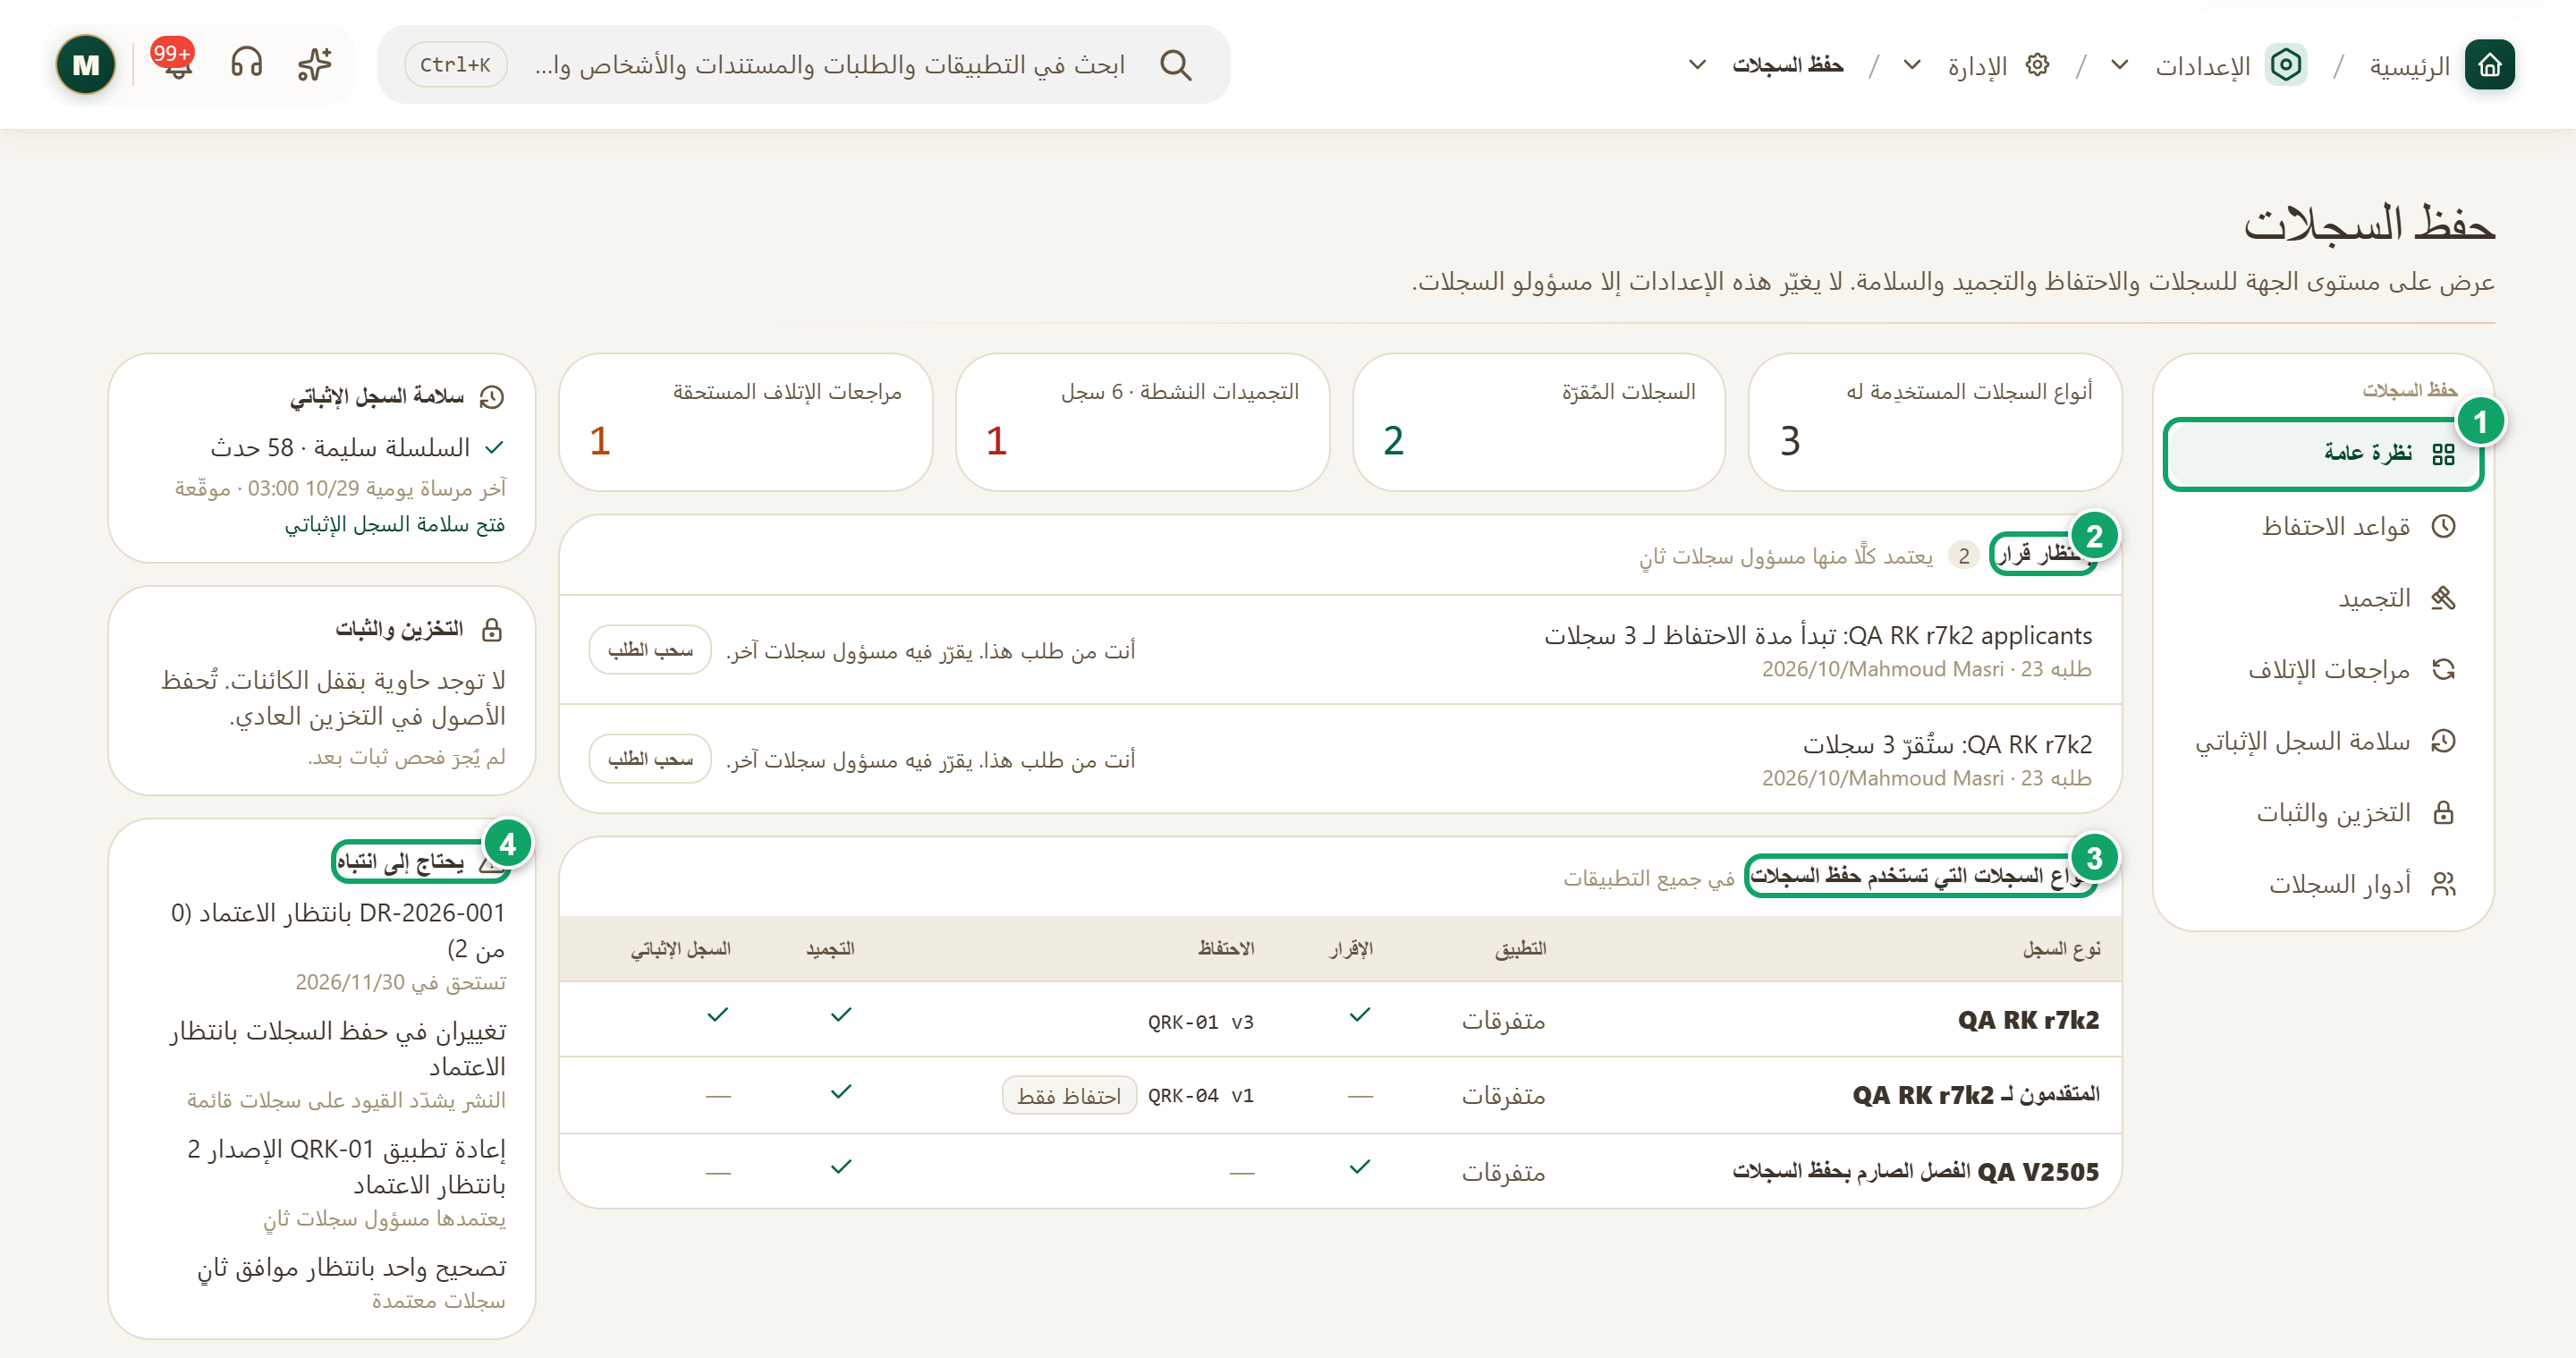
\includegraphics[width=0.95\linewidth,height=0.72\textheight,keepaspectratio]{figures/screens/ch08-record-keeping-ar.png}
\caption{نظرة عامة على حفظ السجلات}
\label{fig:settings-record-keeping-screen}
\shotnote{تجمع النظرة العامة الأرقام الرئيسية وما ينتظر قراراً، فتعرف من أين تبدأ. والبيانات المعروضة بيانات اختبار. ولا يعتمد صاحب الطلب طلبه؛ لذلك يُظهر الصف أنه بانتظار مسؤول سجلات آخر. ① «نظرة عامة». ② «بانتظار قرار». ③ «أنواع السجلات التي تستخدم حفظ السجلات». ④ «يحتاج إلى انتباه».}
\end{figure}

\begin{figure}[H]
\centering
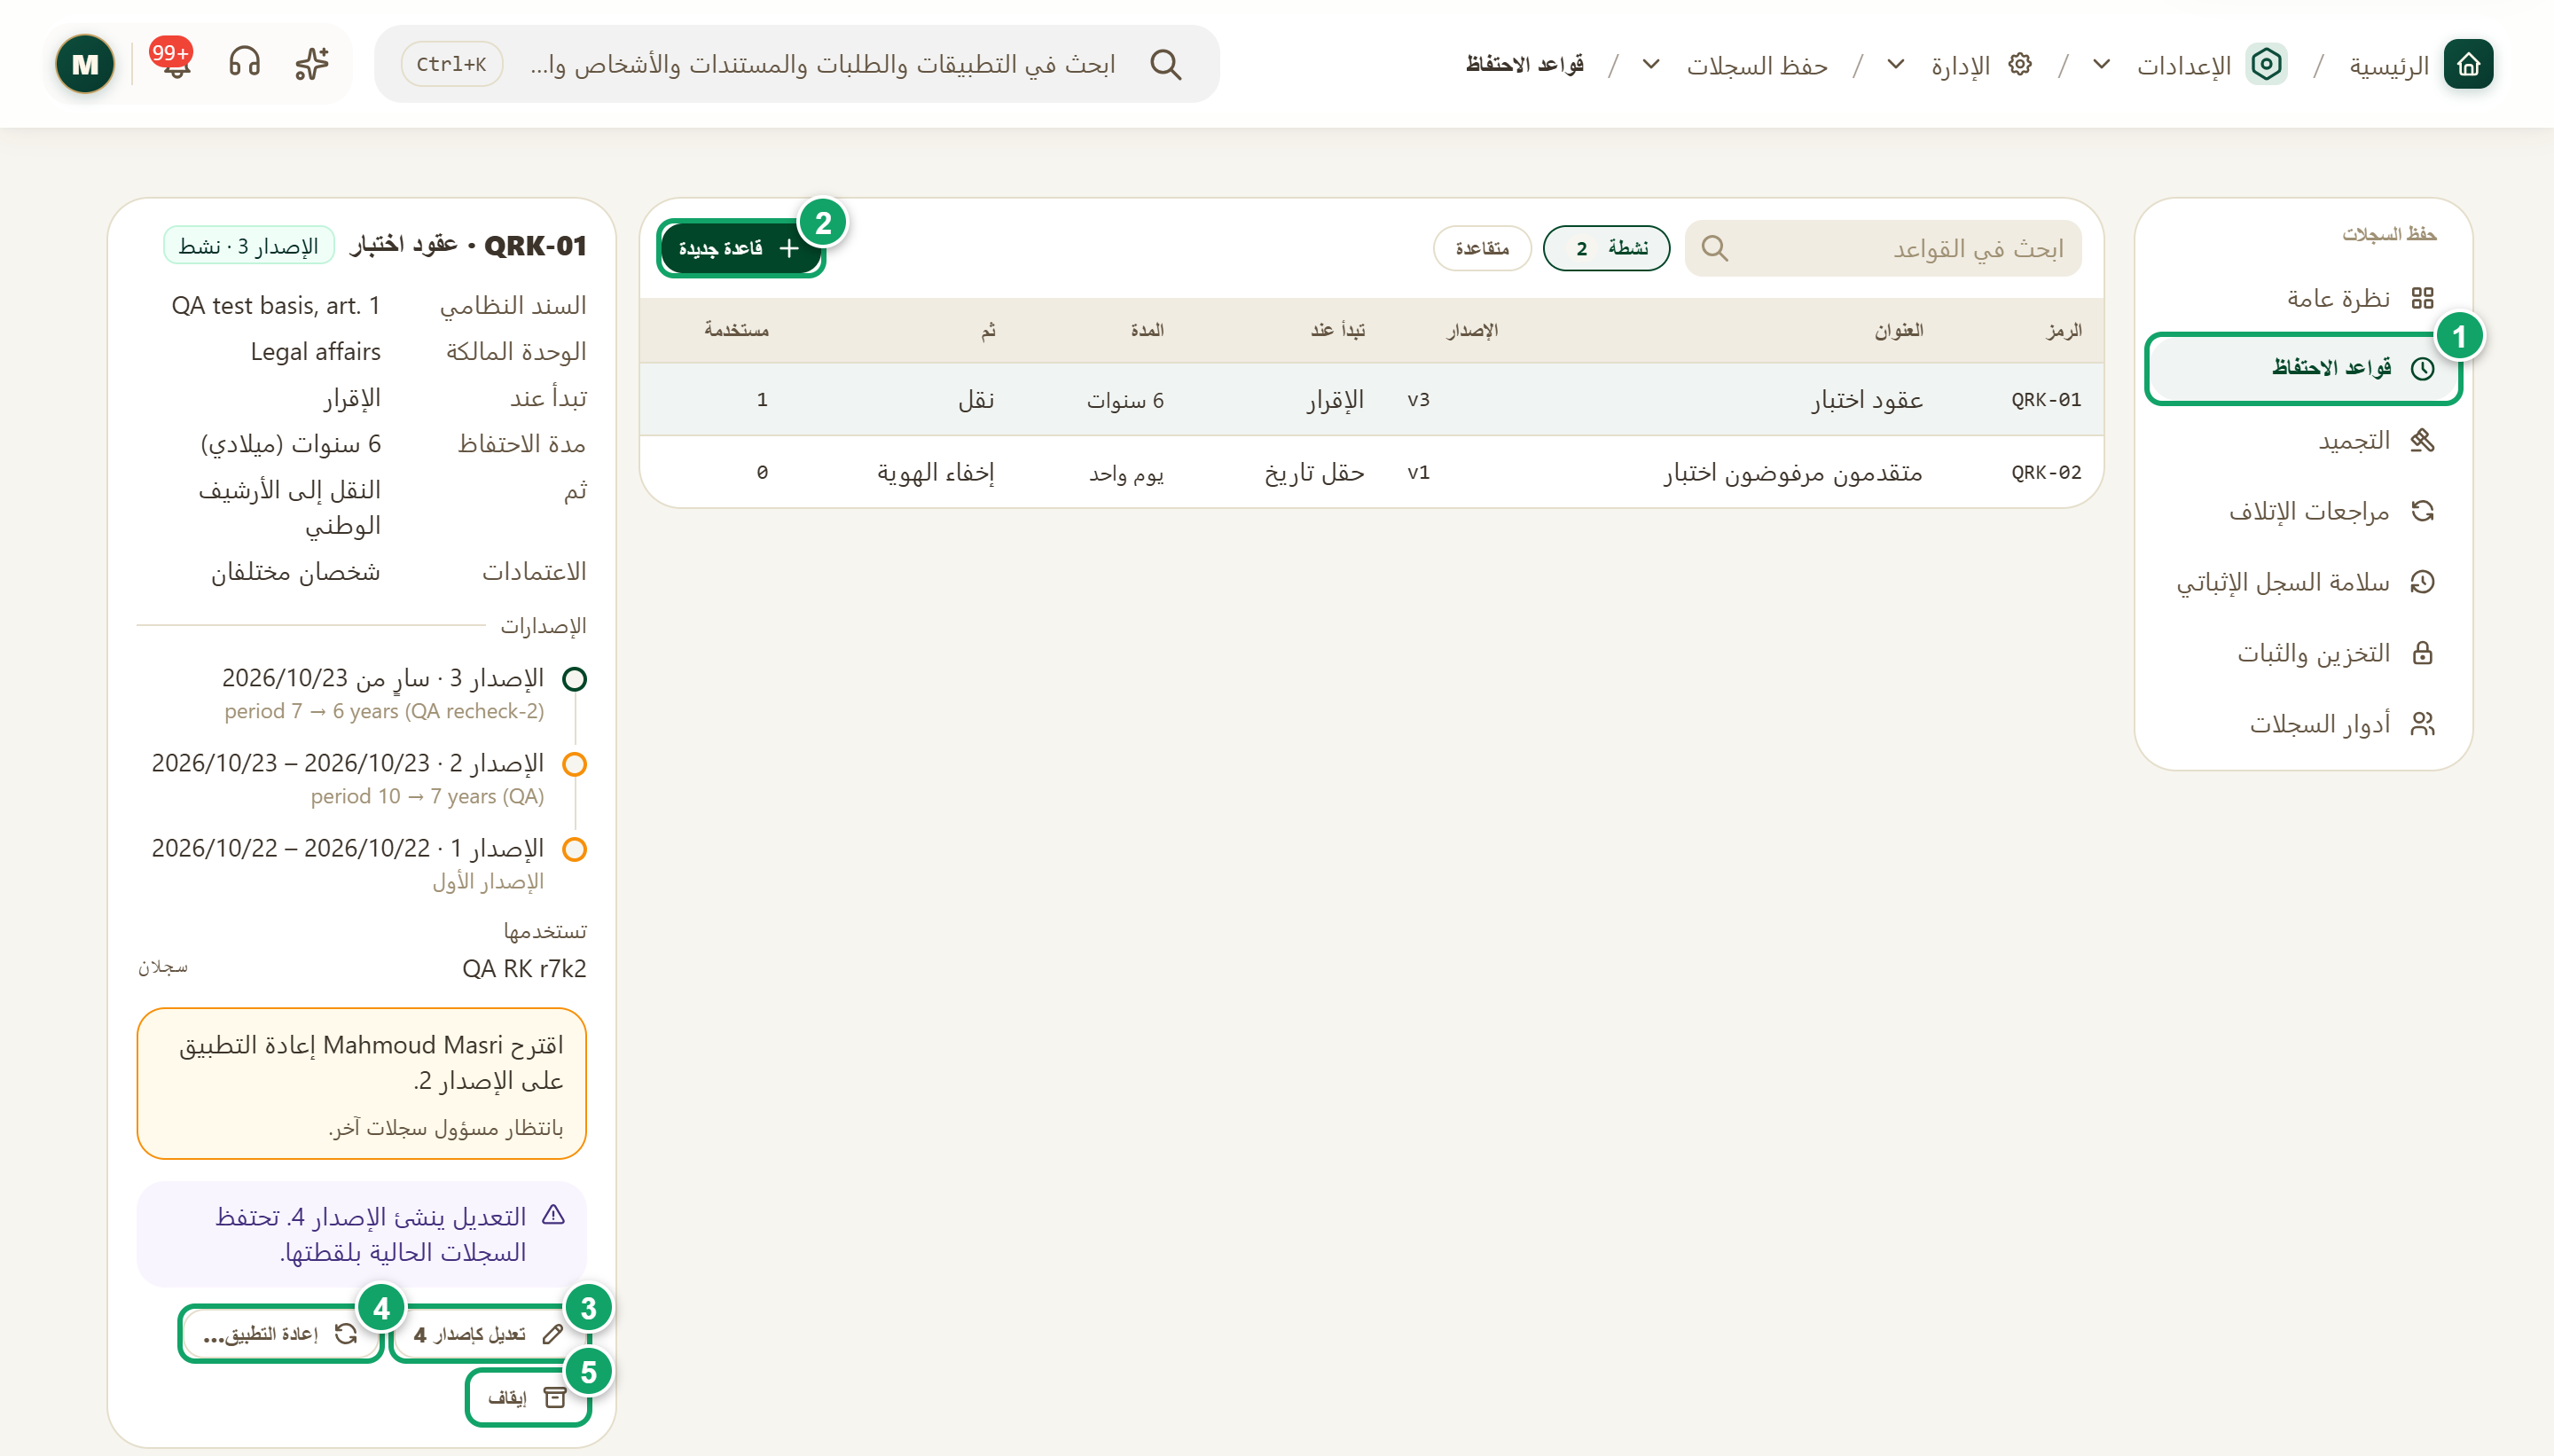
\includegraphics[width=0.95\linewidth,height=0.72\textheight,keepaspectratio]{figures/screens/ch08-record-keeping-rules-ar.png}
\caption{قواعد الاحتفاظ}
\label{fig:settings-record-keeping-rules-screen}
\shotnote{تحدد القاعدة متى تبدأ المدة وكم تطول وماذا يحدث بعدها. وعند تعديلها يُنشأ إصدار جديد، وتحتفظ السجلات الحالية بإصدارها حتى تُعتمد إعادة التطبيق. ① «قواعد الاحتفاظ». ② «قاعدة جديدة». ③ «تعديل كإصدار». ④ «إعادة التطبيق…»: تقترح نقل السجلات الحالية، ويعتمد ذلك مسؤول سجلات آخر. ⑤ «إيقاف»: تمنع السجلات الجديدة من استخدام القاعدة.}
\end{figure}

\begin{figure}[H]
\centering
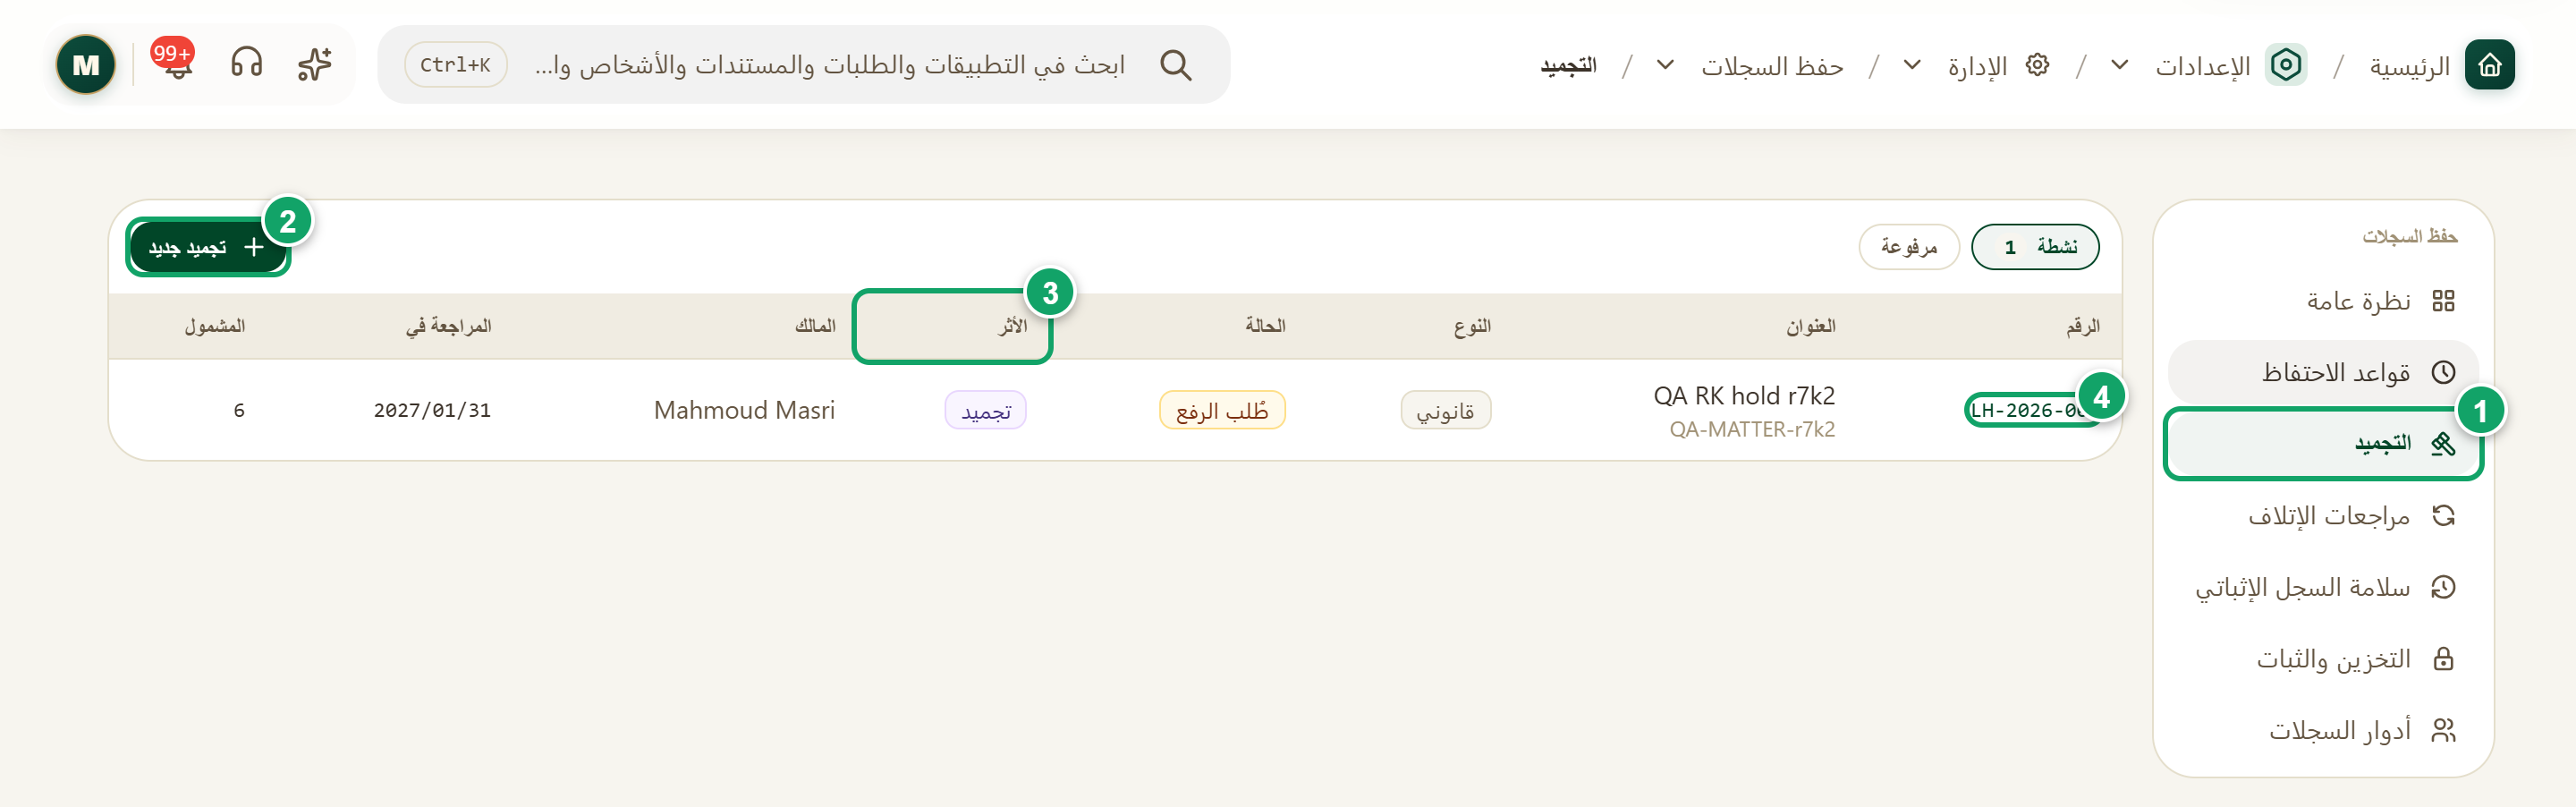
\includegraphics[width=0.95\linewidth,height=0.72\textheight,keepaspectratio]{figures/screens/ch08-record-keeping-holds-ar.png}
\caption{التجميد}
\label{fig:settings-record-keeping-holds-screen}
\shotnote{يعلّق التجميد الإتلاف والحذف عن سجلات محددة، ويُعاد فحص نطاقه كل ليلة وعند كل تعديل. ولا يُرفع إلا بموافقة الشؤون القانونية ومالك التجميد. ① «التجميد». ② «تجميد جديد». ③ «الأثر»: «حفظ» يسمح بالتعديل مع إبقاء كل نسخة، و«تجميد» يمنع التعديل أيضاً. ④ رقم التجميد: يفتح نطاقه وسجلاته.}
\end{figure}

\begin{figure}[H]
\centering
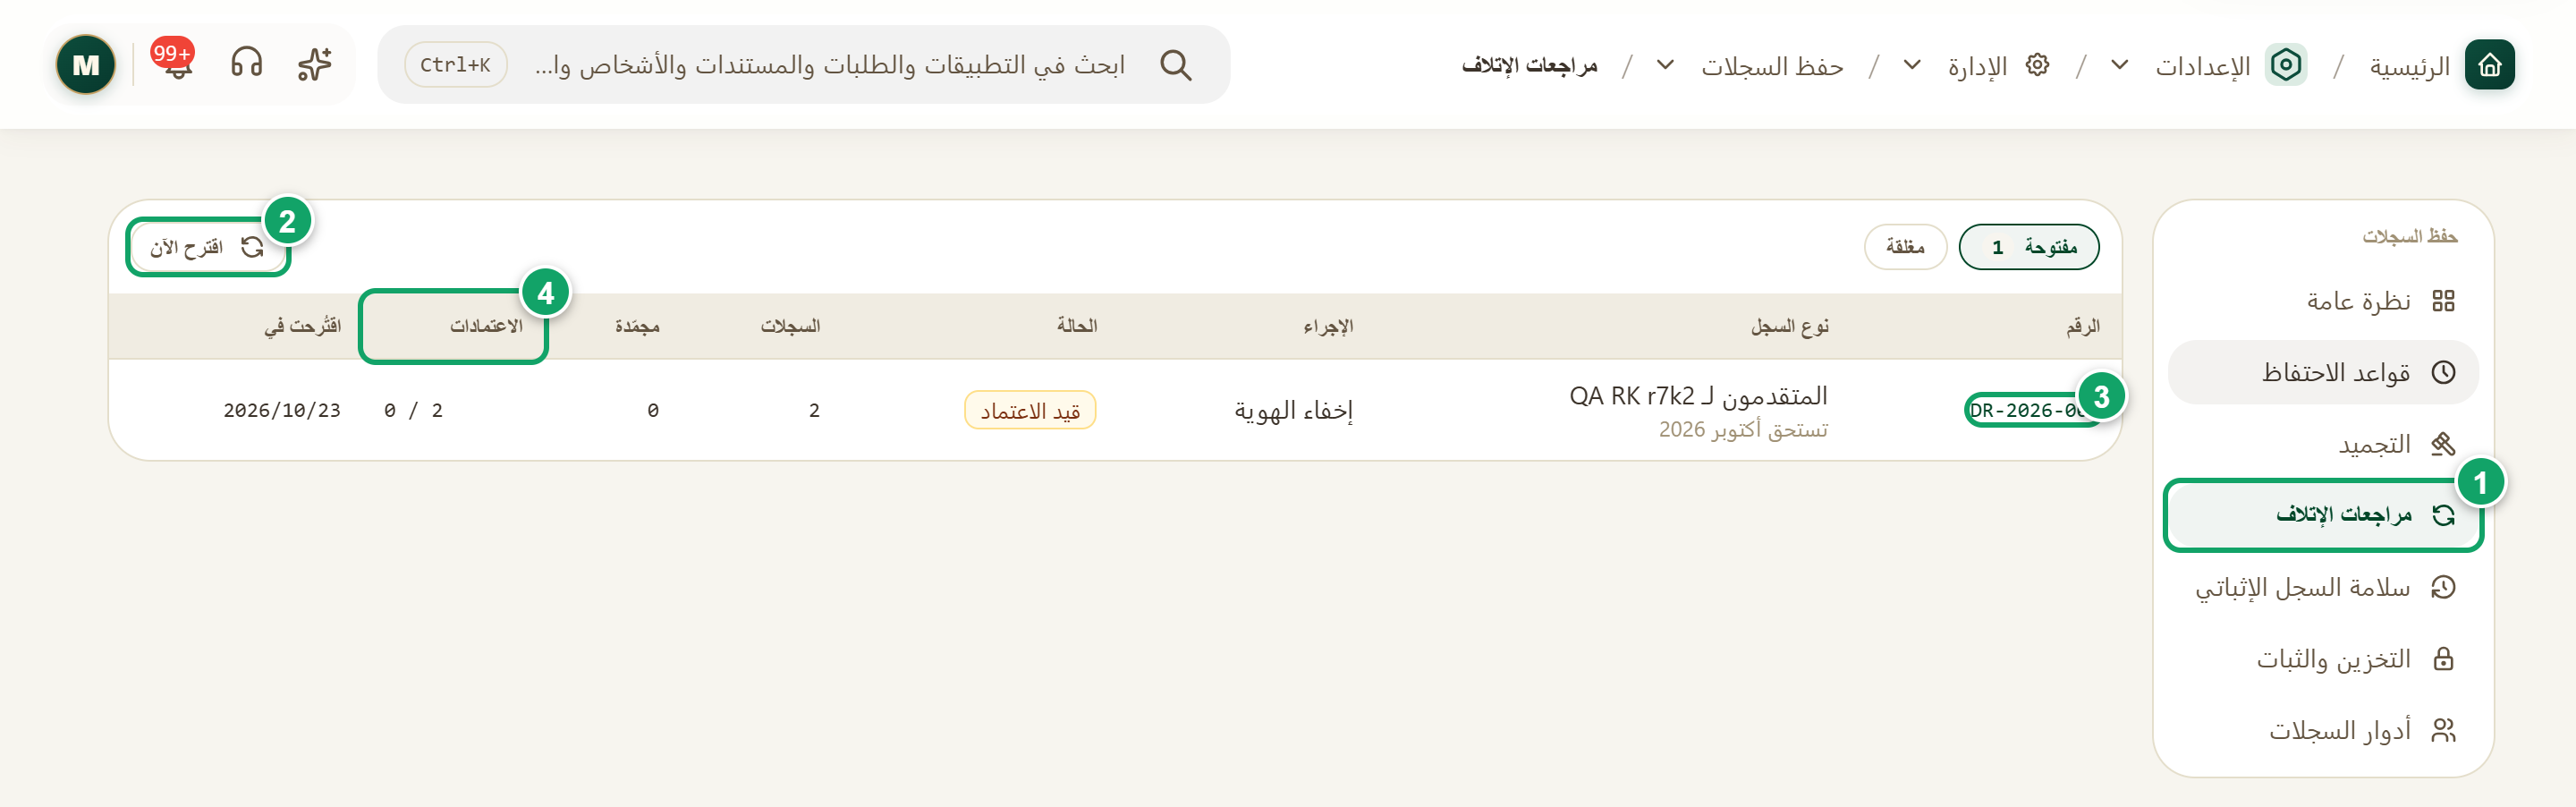
\includegraphics[width=0.95\linewidth,height=0.72\textheight,keepaspectratio]{figures/screens/ch08-record-keeping-disposition-ar.png}
\caption{مراجعات الإتلاف}
\label{fig:settings-record-keeping-disposition-screen}
\shotnote{تجمع المراجعة السجلات المستحقة في طلب واحد يُعتمد قبل التنفيذ. ويقترحها النظام شهرياً، ولا يعتمدها من اقترحها. ① «مراجعات الإتلاف». ② «اقترح الآن»: ينشئ المراجعات المستحقة دون انتظار الموعد الشهري. ③ رقم المراجعة: يفتح سجلاتها واعتماداتها وشهادتها. ④ «الاعتمادات».}
\end{figure}

\begin{figure}[H]
\centering
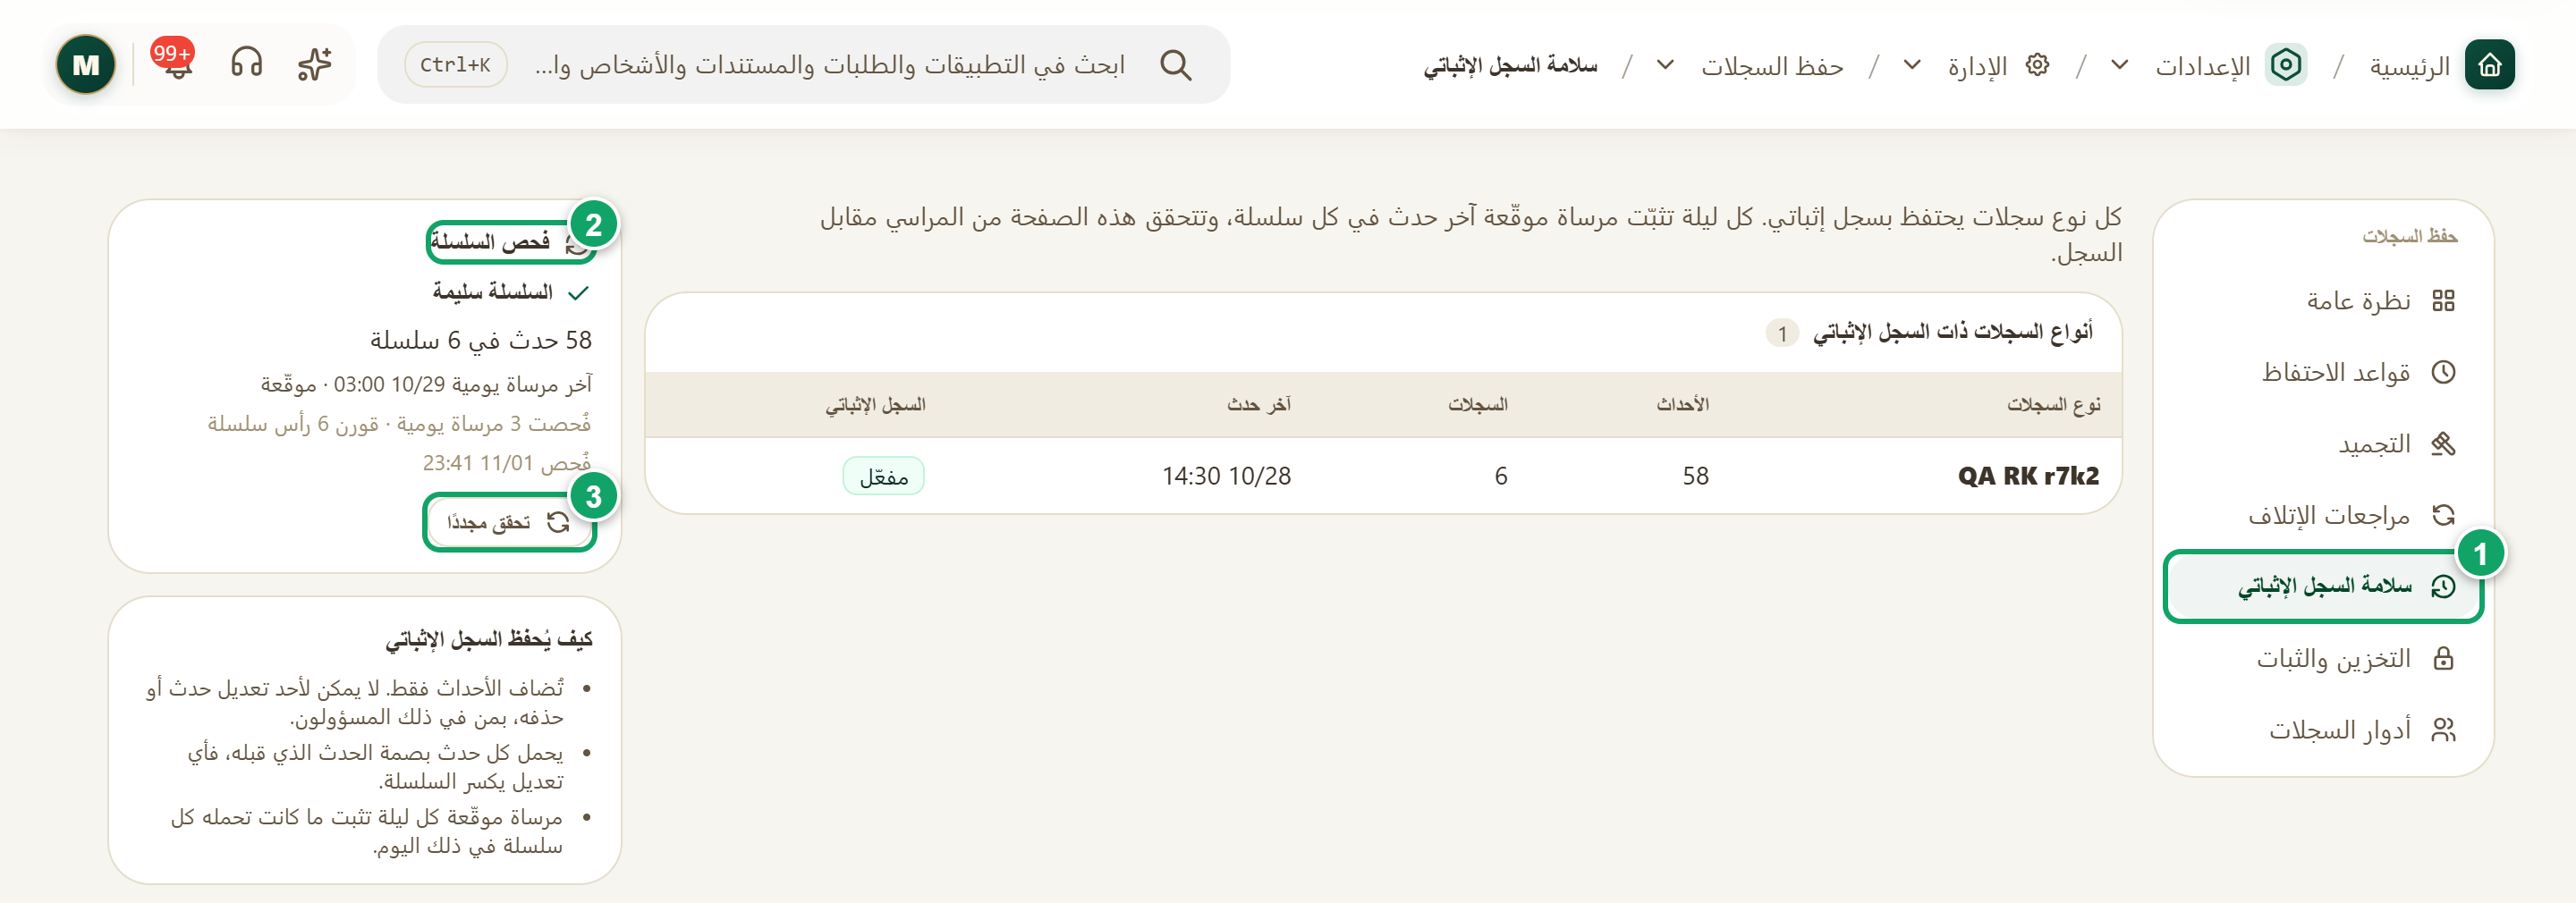
\includegraphics[width=0.95\linewidth,height=0.72\textheight,keepaspectratio]{figures/screens/ch08-record-keeping-ledger-ar.png}
\caption{سلامة السجل الإثباتي}
\label{fig:settings-record-keeping-ledger-screen}
\shotnote{السجل الإثباتي قائمة أحداث لا يُحذف منها شيء ولا يُغيَّر، حتى من المسؤولين. ويرتبط كل حدث بالحدث الذي قبله، فيظهر أي عبث عند الفحص. ① «سلامة السجل الإثباتي». ② «فحص السلسلة»: يعرض نتيجة المقارنة بالنقاط المرجعية الموقعة التي تُسجَّل كل ليلة. ③ «تحقق مجددًا».}
\end{figure}

\begin{figure}[H]
\centering
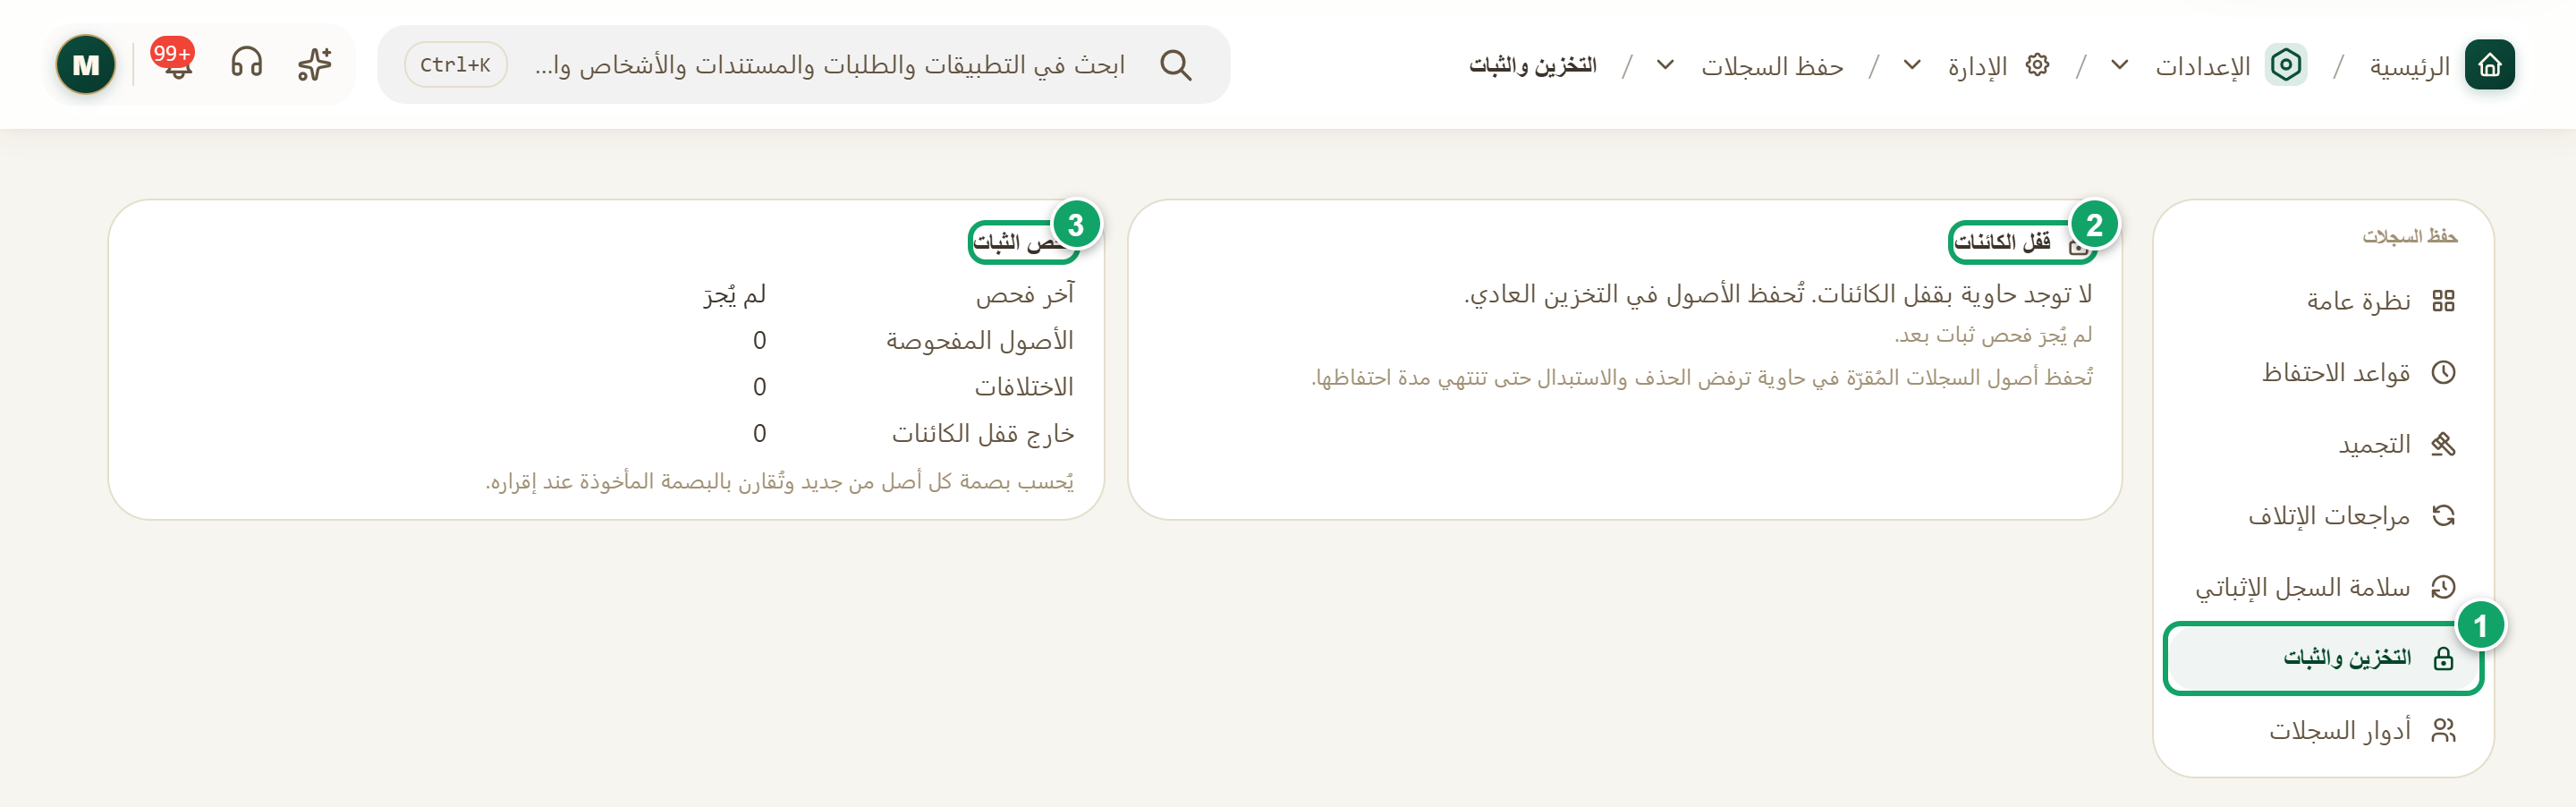
\includegraphics[width=0.95\linewidth,height=0.72\textheight,keepaspectratio]{figures/screens/ch08-record-keeping-storage-ar.png}
\caption{التخزين والثبات}
\label{fig:settings-record-keeping-storage-screen}
\shotnote{تعرض الصفحة حماية الملفات الأصلية للسجلات المقرّة، ويظهر هنا أن مؤسسة الاختبار لم تُعدّ هذه الحماية بعد، وأن أي فحص لم يُجرَ. ① «التخزين والثبات». ② «قفل الكائنات»: تخزين يرفض الحذف والاستبدال حتى تنتهي المدة. ③ «فحص الثبات»: يقارن بصمة كل أصل بما حُفظ عند الإقرار.}
\end{figure}

\begin{figure}[H]
\centering
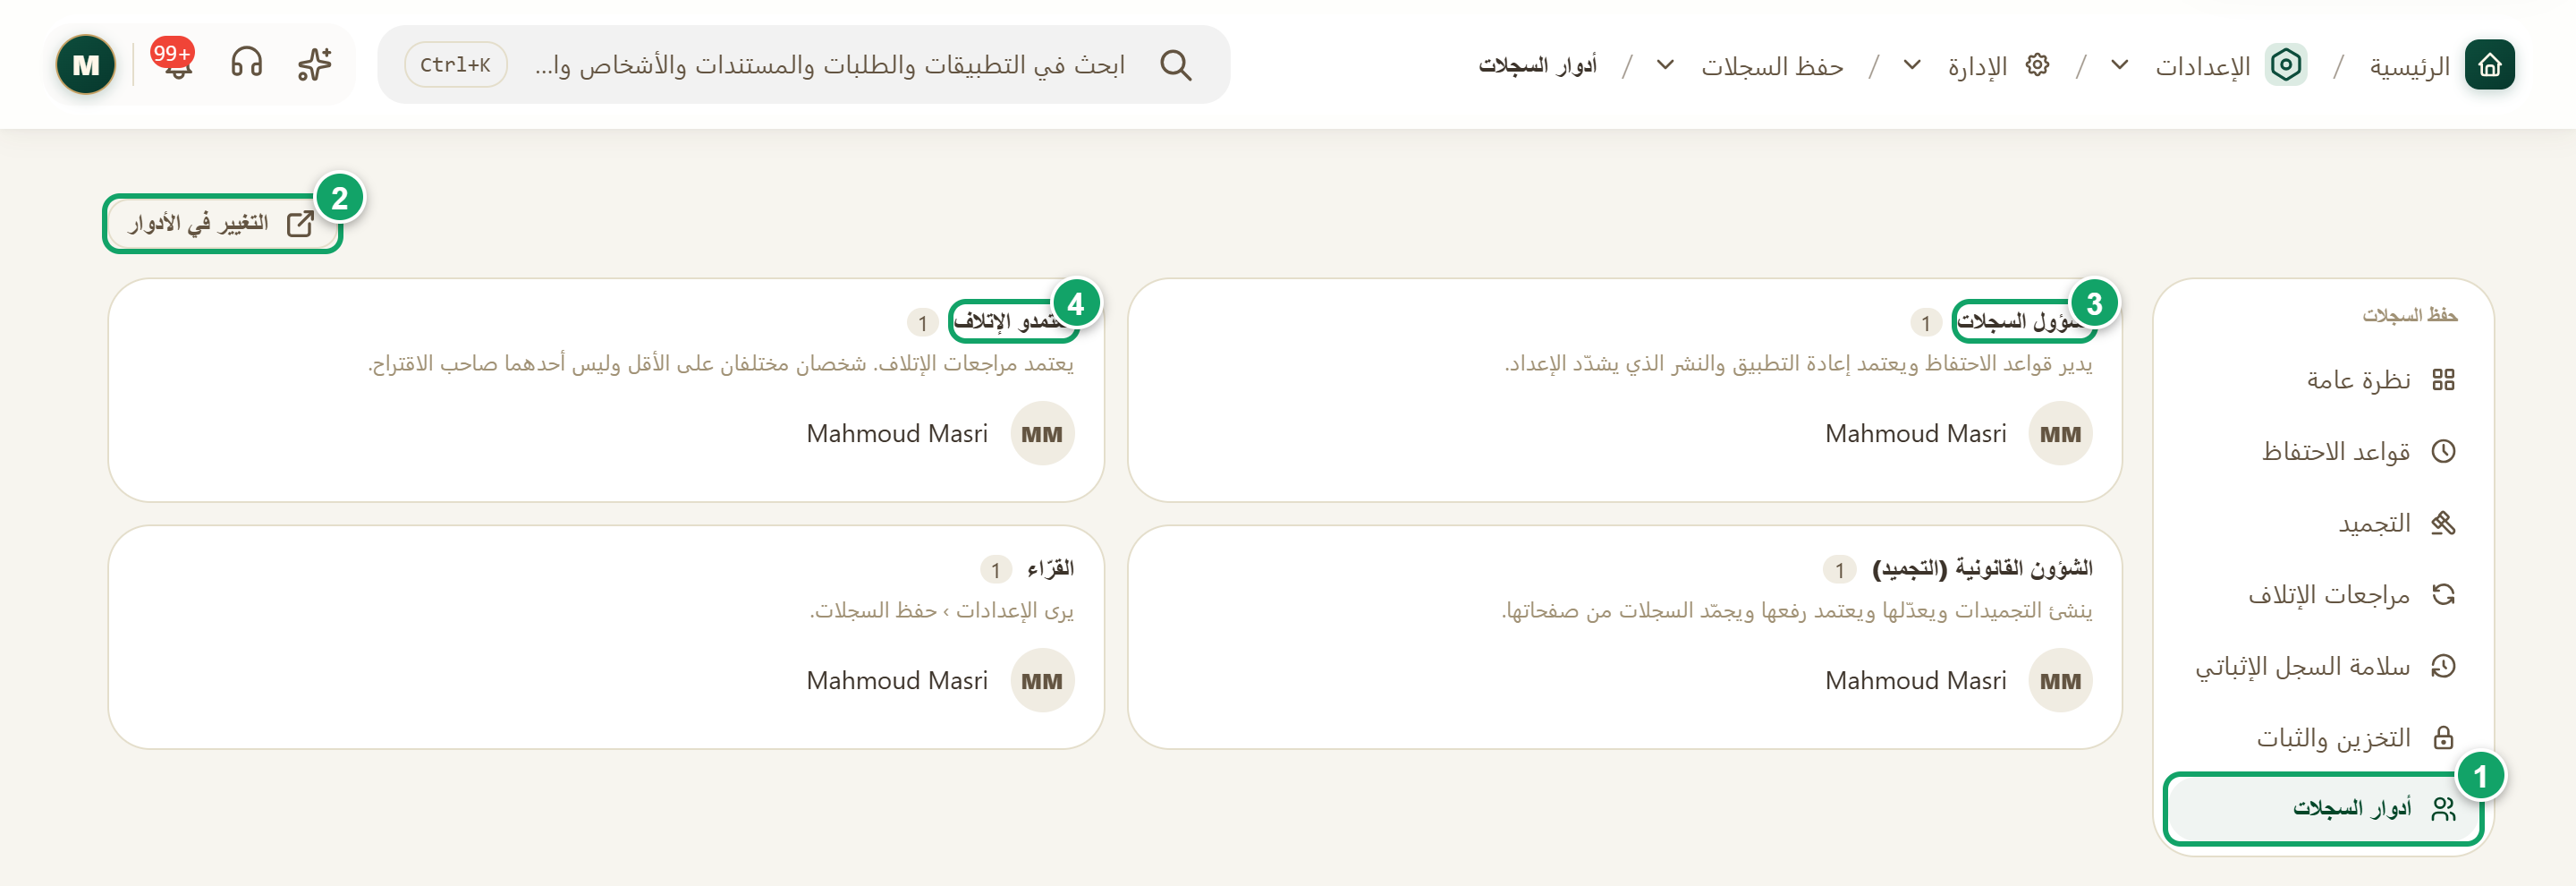
\includegraphics[width=0.95\linewidth,height=0.72\textheight,keepaspectratio]{figures/screens/ch08-record-keeping-roles-ar.png}
\caption{أدوار السجلات}
\label{fig:settings-record-keeping-roles-screen}
\shotnote{تبين الصفحة من يحمل كل مسؤولية، لكنها لا تغيّرها مباشرة. ويفيد فصل الأدوار في منع شخص واحد من اقتراح الإتلاف واعتماده. ① «أدوار السجلات». ② «التغيير في الأدوار»: ينقلك إلى صفحة الأدوار. ③ «مسؤول السجلات». ④ «معتمدو الإتلاف».}
\end{figure}

\begin{table}[H]
\centering
\caption{ماذا تسجل في حفظ السجلات؟}
\label{tab:settings-record-keeping-fields}
\begin{tabularx}{\linewidth}{R{4.2cm} Y}
\rcHeaderRow
\thh{القسم} & \thh{ماذا تسجل أو تقرأ؟}\\
«قواعد الاحتفاظ» & الرمز، و«السند النظامي»، والعنوان، و«الوحدة المالكة»، و«سارية من»، و«تبدأ عند»، و«مدة الاحتفاظ» والوحدة والتقويم، و«ثم»، و«الاعتمادات المطلوبة» من شخصين إلى خمسة، و«ما الذي تغيّر».\\
«التجميد» & النوع، والعنوان، و«القضية»، و«المراجعة في»، والسبب، و«المالك»، و«الوحدة المالكة»، و«الأثر»، و«الأمناء» وهم الأعضاء الذين يشمل التجميد سجلاتهم وملفاتهم، والنطاق.\\
«مراجعات الإتلاف» & السجلات والمستبعد منها والاعتمادات. ويمكن إزالة سجل قبل بدء الاعتمادات، وتصدر الشهادة بعد التنفيذ.\\
«سلامة السجل الإثباتي» & عدد الأحداث، وآخر مرساة موقعة، وأنواع السجلات التي تحتفظ بسجل إثباتي.\\
«التخزين والثبات» & حالة قفل الكائنات، وآخر فحص، والأصول المفحوصة، والاختلافات.\\
«أدوار السجلات» & الأعضاء في «مسؤول السجلات» و«معتمدو الإتلاف» و«الشؤون القانونية (التجميد)» و«القرّاء».\\
\end{tabularx}
\end{table}

\begin{enumerate}
\item افتح «الإعدادات» ثم «حفظ السجلات»، وابدأ من «نظرة عامة» بقراءة «يحتاج إلى انتباه».
\item لإضافة قاعدة، افتح «قواعد الاحتفاظ» واضغط «قاعدة جديدة»، ثم املأ الحقول واضغط «إنشاء القاعدة».
\item لوضع تجميد، افتح «التجميد» واضغط «تجميد جديد»، واختر النوع والأثر والنطاق، ثم اضغط «إنشاء التجميد».
\item لمراجعة الإتلاف، افتح المراجعة، وافحص سجلاتها، ثم اضغط «اعتماد» أو «رفض» إذا كنت من المعتمدين.
\item لرفع تجميد، افتحه واضغط «طلب الرفع»؛ فيُرفع بعد موافقة مالكه والشؤون القانونية.
\end{enumerate}

\textbf{تحقق:} تظهر القاعدة في قائمة «نشطة»، ويظهر التجميد برقمه وعدد السجلات المشمولة. وتتحرك مراجعة الإتلاف عبر مراحلها، ولا تُنفَّذ قبل اكتمال الاعتمادات. وإذا لم تجد نوع سجلاتك في النظرة العامة، ففعّل حفظ السجلات له من أداة البناء.
